\newpage
\section{Arbeitspakete}
Dieser Abschnitt beschreibt die Unterteilung des Projekts in Arbeitspakete und wie die Gruppenmitglieder die zugeteilten Arbeitspakte abarbeitet haben. Es wird auch auf den unvorhergesehenen Arbeitsbereitschaftsmangel der Gruppenmitglieder Herr Gregarek und Herr Dück eingegangen.

\subsection{Einteilung der Arbeitspakete}
Zunächst wurden die Arbeitspakete aus der Anforderungsanalyse abgeleitet. Aus dieser Ableitung sind folgende Arbeitspakete definiert worden:
\begin{enumerate}
	\item Entwicklung des grundlegenden Webseitendesigns für Desktop-Rechner
	\item Anpassung des Designs für mobile Geräte
	\item Entwicklung der Webseitennavigationsleiste
	\item Entwicklung der inhaltlichen Seiten des Webshops:
	\begin{itemize}
		\item Startseite
		\item Produktseite
		\item Rechtliche Seiten:
		\begin{itemize}
			\item[$\diamond$] Impressum
			\item[$\diamond$] Datenschutz
			\item[$\diamond$] AGB
		\end{itemize}
	\end{itemize}
	\item Entwicklung einer Schnittstellendatenbank zum Datenaustausch zwischen Webshop und SAP-System:
	\begin{itemize}
		\item Ansprechpartner der SAP-Gruppe für die Schnittstelle zum Webshop
		\item Entwurf von Tabellen für die Datenhaltung des Webshops 
	\end{itemize}
	\item Registrierungs- und Anmeldungsfenster designen und programmieren
	\begin{itemize}
		\item Möglichkeit den Kunden bieten die Anmeldeinformationen später verändern zu können
	\end{itemize}
	\item Entwickeln einer Suchfunktion:
	\begin{itemize}
		\item Autovervollständigung
		\item Erweiterte Suchfunktion, wo die Suche genauer eingegrenzt werden kann
		\item Auflistung der Suchergebnisse
	\end{itemize}
	\item Warenkorb
	\begin{itemize}
		\item Auflistung der Produkte, die sich im Warenkorb befinden
		\item Formular mit Mengenfeld, um ein Produkt in den Warenkorb zu packen
		\item Möglichkeit zur nachträglichen Änderung der Produkte im Warenkorb:
		\begin{itemize}
			\item[$\diamond$] Änderung der Bestellmenge
			\item[$\diamond$] Entfernen des Produkts aus dem Warenkorb
		\end{itemize}
	\end{itemize}
	\item Bestellvorgang:
	\begin{itemize}
		\item Bestellroutine mit folgenden Schritten:
		\begin{itemize}
			\item[$\diamond$] Wahl der Versandart
			\item[$\diamond$] Nachträglichen Änderung der Bestellmenge der Produkte
			\item[$\diamond$] Wahl Zahlungsart
			\item[$\diamond$] Wahl Lieferadresse
			\item[$\diamond$] Bestellübersichtseite zur Kontrolle vor den Absenden der Bestellung
		\end{itemize}
		\item Einsicht des aktuellen Status der Bestellung
		\item Möglichkeit die Bestellung zu stornieren
	\end{itemize}
	
	\item Erstellung eines Marketing Mix
	\item Bewertungsfunktion von Artikel (mit Kommentarfunktion)
	\item Email-Versand
	\begin{itemize}
		\item Klasse für den Email-Versand entwerfen
		\item Designen der Bestätigungs-Emails
	\end{itemize}					 
\end{enumerate}

Die oben genannten Arbeitspakete hat sich die Gruppe untereinander aufgeteilt. Stefan Schnürer hat Arbeitspakete 1,3 und 4 übernommen. Benedikt Brüntrup übernahm die Arbeitspakete 5, 6 und 7. Michael Dück hatte sich bereit erklärt die Arbeitspakte 2, 11 und 12 zu bearbeiten. Raphael wollte die Arbeitspakete 8, 9 und 10 abarbeiten.


%Nachfolgend soll auf die einzelnen Zwischenschritte des Projekts eingegangen werden.Das Projekt beginnt mit der Projektplanung. Hierbei werden die Arbeitspakete definiert und an den entsprechenden Gruppenmitgliedern verteilt. Pro Arbeitspaket wird eine Bearbeitungsdauer von zwei Wochen festgelegt. Es wird ein Projektzeitplan sowie eine Risikoanalyse erstellt. Im Anschluss daran werden grobe Design Entwürfe für die Homepage erstellt. Es wird sich für den Design Entwurf von Herrn Brüntrup entschieden. Die Homepage wird in einem matten Grün-Ton designt, um den Kunden die Umweltaspekte von Fahrrädern zu verdeutlichen.
%\textbf{Was machen Herr Gregarek und Herr Dück?}

\newpage
\subsection{Arbeitspaket von Herrn Schnürer}

Dieser Abschnitt beschreibt den Aufgabenteil von Herrn Schnürer und wie dieser den Seitenprototyp, den statischen und dynamischen Inhalt und Aufbau der Seite sowie die CSS-Datei zur Anzeige des Webshops auf Desktop Rechnern entwickelt hat.


\subsubsection{Arbeitspaket 1: Erster Seitenprototyp}

Der erste Prototyp der Seite basiert auf den Standardverfahren einer Webseite. Dabei wird der Inhalt der Seite in HTML geschrieben, während eine CSS Datei für das Seitenlayout der Webseite verantwortlich ist. \textit{Abbildung 11} zeigt einen ersten groben Designentwurf der Startseite, anhand dessen orientiert sich auch der erste Seitenprototyp von Herrn Schnürer:

\begin{figure}[H]
\begin{center}
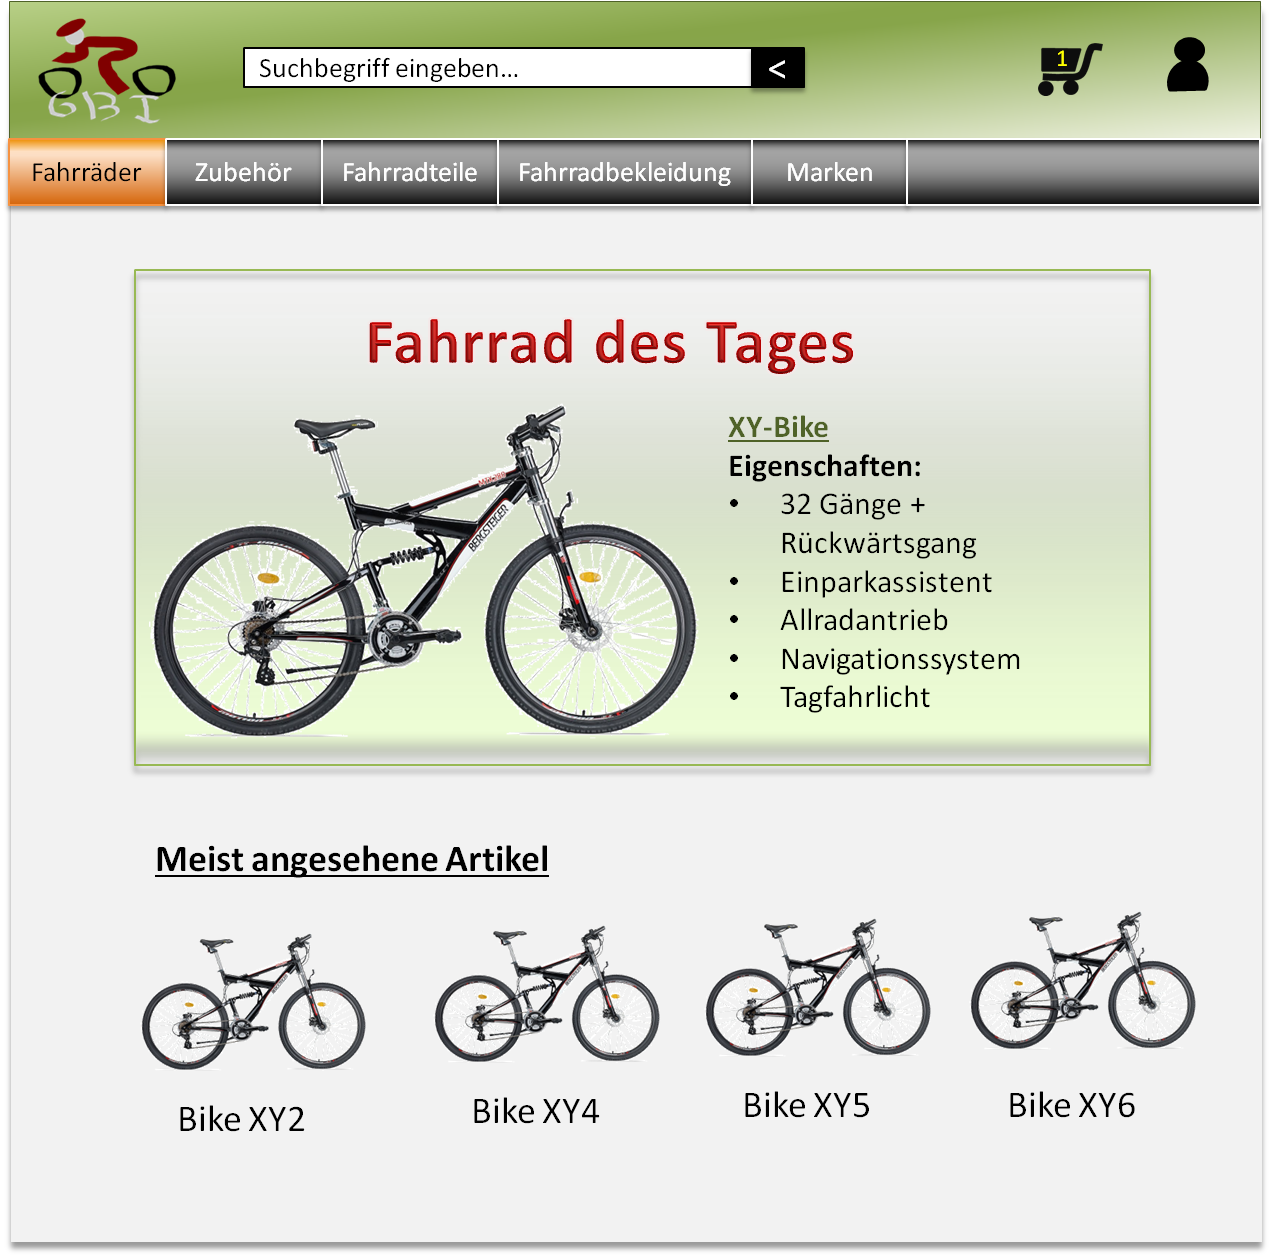
\includegraphics[width=8cm]{Bilder/Abbildung2-GroberDesignEntwurfDesWebshops.png}
\end{center}
\caption{Erster grober Designentwurf der Startseite}
\end{figure}


\subsubsection{Arbeitspaket 1 und 4: Startseite des Webshops}

Die Startseite wird zunächst mit zwei einfachen Artikeln versehen. Sie sollen eine grobe Vorstellung liefern, wie die fertige Startseite aussehen könnte.

\subsubsection{Arbeitspaket 3: Seitennavigation}

In den darauf folgenden Wochen liegt der Fokus auf die Seitennavigation in der Kopfzeile (nachfolgend Header) der Seite. Die Seitennavigation wird mithilfe von CSS an den Designentwurf angepasst. Es werden die Hauptkategorien \glqq{Fahrräder}\grqq{}, \glqq{Zubehör}\grqq{}, \glqq{Fahrradteile}\grqq{}, \glqq{Fahrradbekleidung}\grqq{}, \glqq{Marken}\grqq{} und eine Rubrik \glqq{HowTo}\grqq{} angezeigt. Letztere verlinkt auf eine Internetquelle, mit dessen Hilfe die Seitennavigation umgesetzt wurde. Diese Kategorie dient den anderen Gruppenmitgliedern als Referenz und wird in späteren Versionen des Webshops wieder entfernt. Fährt der Nutzer mit der Maus über die Kategorie \glqq{Fahrräder}\grqq{} öffnet sich ein Drop-Down-Menü, welches den Nutzer verschiedene Fahrradmodelle auswählen lässt. Die komplette Seitennavigation wurde in CSS3 umgesetzt. CSS3 kann von nahezu jeden aktuellen Browser gelesen werden und bietet zudem den Vorteil, dass der entsprechende Code in der bisherigen CSS-Datei eingefügt werden kann. Da CSS3 unabhängig von Java Script ist, lässt sich die Seite zudem problemlos bedienen, wenn Java Script auf den jeweiligen Browsern deaktiviert ist. Dies begründet die Entscheidung CSS3 für die Seitennavigation zu verwenden.
\\
\textit{Abbildung 12} und \textit{13} zeigen den bisherigen Seitenprototypen. \textit{Quellcode 1} veranschaulicht die Umsetzung des Dropdown-Menüs in CSS:

\begin{figure}[H]
\begin{center}
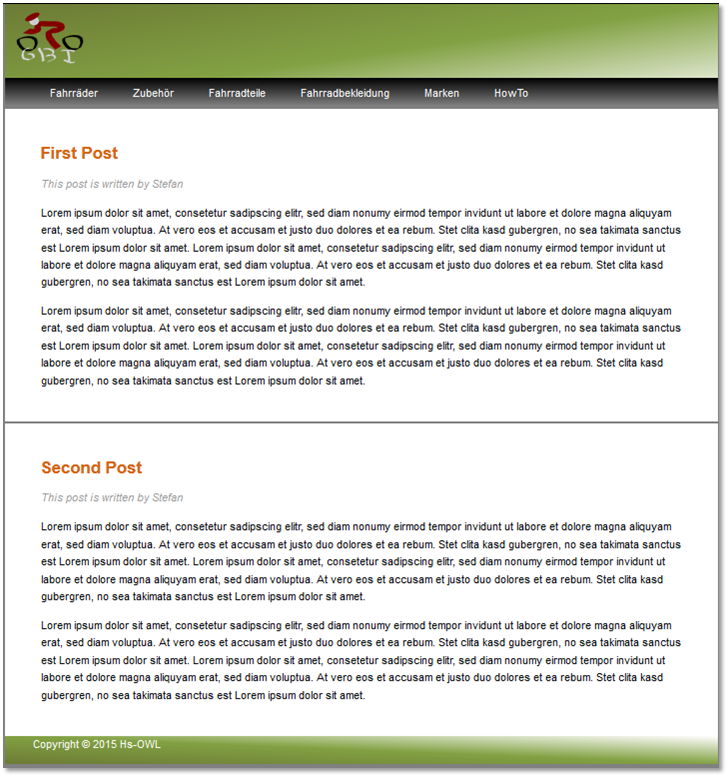
\includegraphics[width=150mm]{Bilder/Abbildung3-Seitenprototyp.png}
\end{center}
\caption{Seitenprototyp}
\end{figure}


\begin{figure}
\begin{center}
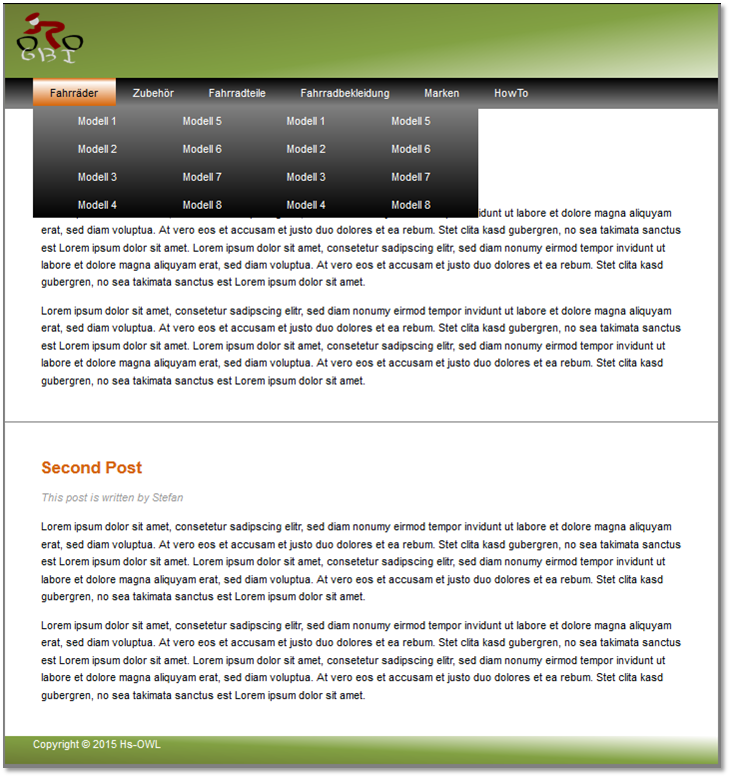
\includegraphics[width=150mm]{Bilder/Abbildung4-SeitenprototypMitDropDownMenue.png}
\end{center}
\caption{Seitenprototyp mit Drop-Down-Menü}
\end{figure}

\newpage
\begin{center}
	\begin{lstinputlisting}[language=CSS, caption={Auszug aus der CSS Datei - Die Seitennavigation}]
		{Quellcode/statischeNavigation.css}
	\end{lstinputlisting}
\end{center}


%Ein paar Wochen später wird sich dazu entschlossen das Programm „Eclipse“ zum Programmieren des Webshops zu nutzen. Das Programm bietet neben einer Autovervollständigung und der Unterstützung mehrerer Programmiersprachen noch zusätzlich den Vorteil, dass es durch Plug-Ins erweiterbar ist. So lässt sich „Eclipse“ durch das Plug-In „GitHub“ erweitern. „GitHub“ ist eine Cloud basierte Lösung zum gemeinsam bearbeiten von Programmcode. Das komplette Projekt wird dabei auf einen Server hochgeladen. Jedes Gruppenmitglied, das einen Acount bei „GitHub“ erstellt hat, kann dem Projekt beitreten, indem es bei den Gruppen- Administrator um Erlaubnis bittet. Dadurch kann ein Dokument von mehreren Gruppenmitgliedern gemeinsam bearbeitet werden. So entstehen mehrere Versionen von einem Dokument, die anschließend wieder zu einem Dokument zusammengefügt werden können.%

\subsubsection{Arbeitspaket 4: Weitere Arbeiten an der Startseite des Webshops}

Im Laufe der nächsten Woche wird die Startseite des Webshops gemäß dem Designentwurfs erstellt (siehe \textit{Abbildung 14}). Auf der Startseite ist das \glqq{Angebot des Tages}\grqq{} zu sehen. Es gibt eine Kurzbeschreibung zu dem Artikel mit den wichtigsten Eigenschafen. Der untere Teil der Startseite zeigt die meist angesehenen Artikel des Nutzers an.

\begin{figure}[H]
\begin{center}

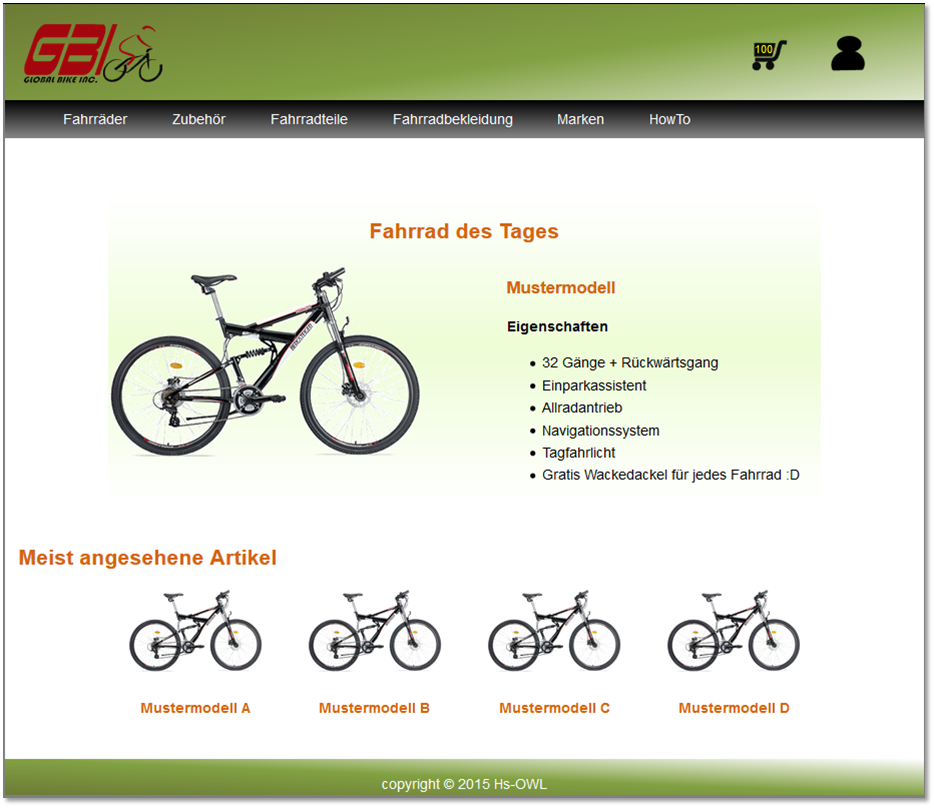
\includegraphics[width=10cm]{Bilder/Abbildung5-StartseiteDesWebshops.png}
\end{center}
\caption{Startseite des Webshops}
\end{figure}


\subsubsection{Arbeitspaket 4: Rechtsschutz}

In den nächsten Tagen wird das Thema Rechtsschutz behandelt. Dem Webshop werden ein Impressum, die AGB sowie Hinweise zum Datenschutz hinzugefügt:

\begin{figure}[H]
\begin{center}
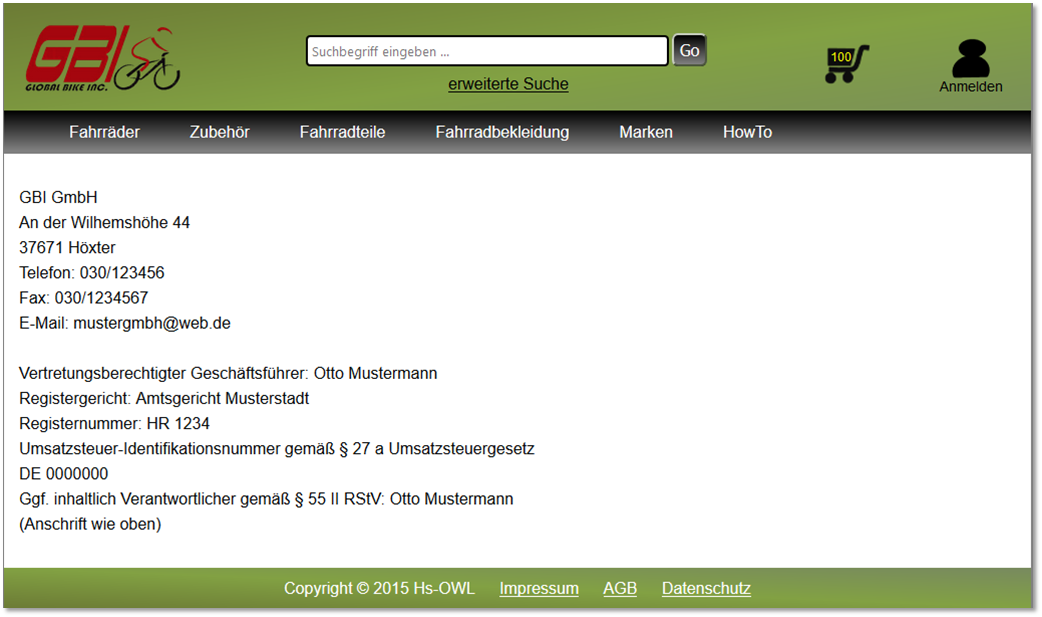
\includegraphics[width=10cm]{Bilder/Abbildung6-ImpressumDesWebshops.png}
\end{center}
\caption{Impressum des Webshops}
\end{figure}

\begin{figure}
\begin{center}
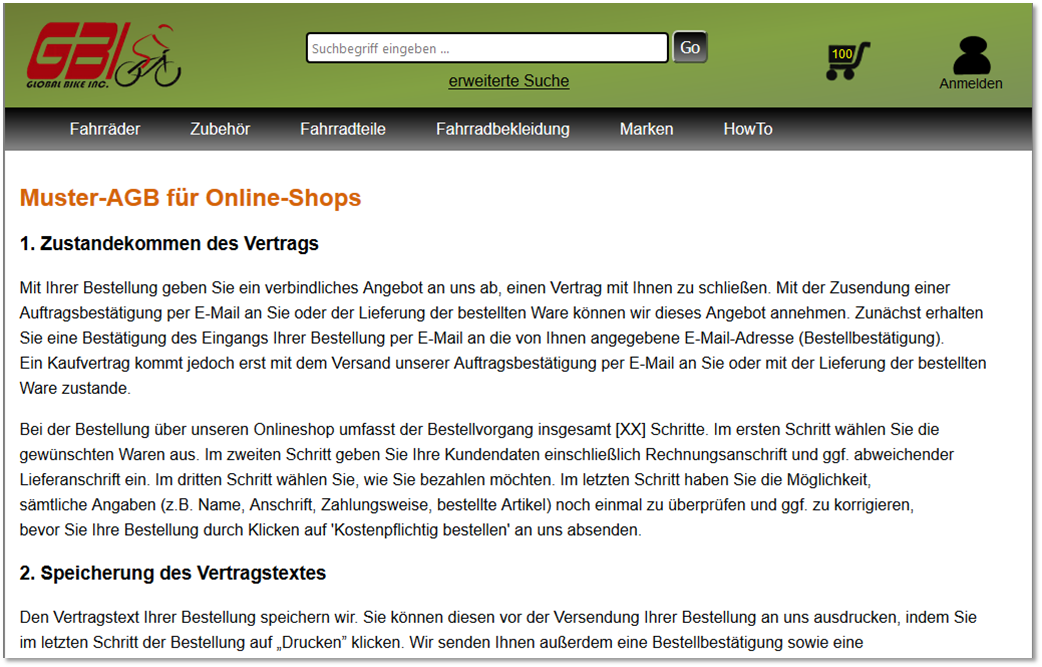
\includegraphics[width=10cm]{Bilder/Abbildung7-AGBDesWebshops.png}
\end{center}
\caption{AGB des Webshops}
\end{figure}

\begin{figure}
\begin{center}
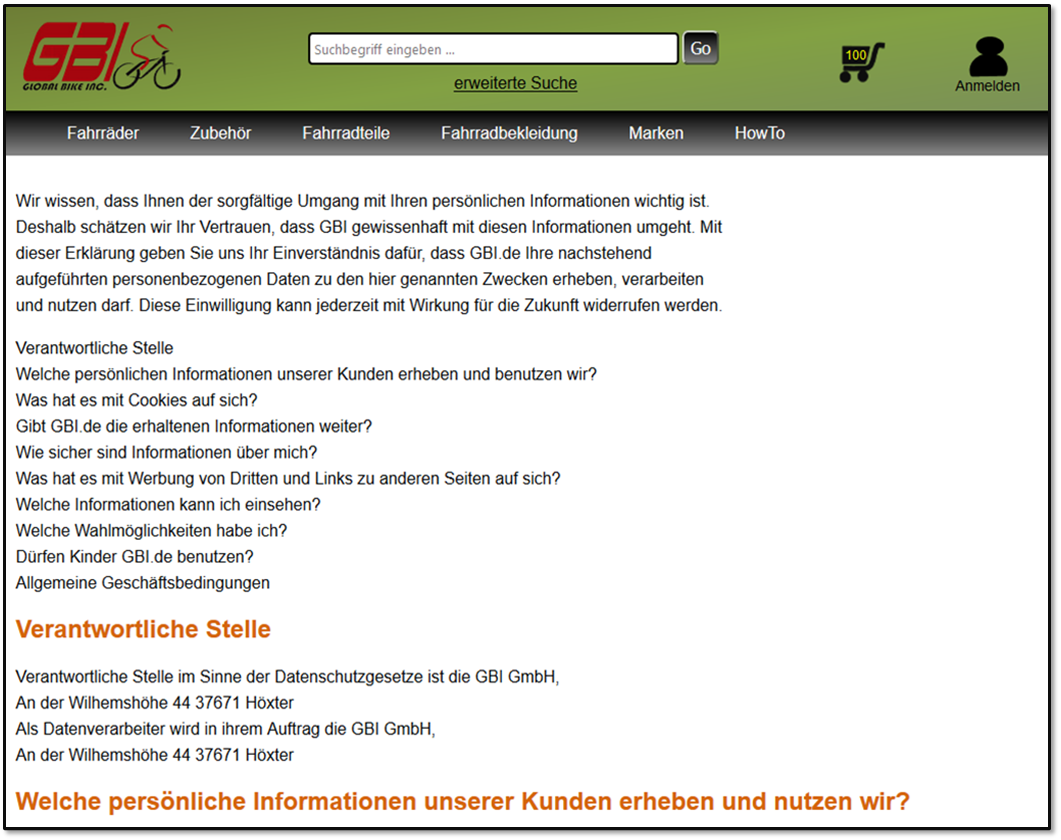
\includegraphics[width=10cm]{Bilder/Abbildung8-DatenschutzDesWebshops.png}
\end{center}
\caption{Datenschutz des Webshops}
\end{figure}

\newpage
\subsubsection{Arbeitspaket 3: Dynamische Seitennavigation}

In den nächsten Wochen wird der statische Inhalt des Webshops durch dynamischen Inhalt ersetzt. Das bedeutet, dass die Daten fortan aus einer Datenbank geladen werden. Diese Datenbank wird mit der Datenbank aus dem SAP- System synchronisiert. Zunächst wird die Navigation des Webshops durch dynamische Inhalte ersetzt. Wird nun eine neue Haupt- oder Unterkategorie hinzugefügt oder entfernt, ändert sich die Navigation entsprechend. Zum besseren Verständnis ein kurzes Beispiel: Angenommen die GBI würde jetzt auch Helmkameras anbieten, so würde in der Datenbank eine neue Kategorie \glqq{Helmkameras}\grqq{} erstellt und zur ihr Kameramodelle von \glqq{GoPro}\grqq{} und \glqq{Rollei}\grqq{}. Die Navigation hätte jetzt die Hauptkategorien \glqq{Fahrräder}\grqq{}, \glqq{Zubehör}\grqq{}, \glqq{Fahrradteile}\grqq{}, \glqq{Fahrradbekleidung}\grqq{} und die Hauptkategorie \glqq{Helmkameras}\grqq{}. Unter letzterer würden die beiden Unterkategorien \glqq{GoPro}\grqq{} und \glqq{Rollei}\grqq{} aufgeführt. \textit{Abbildung 18} zeigt die dynamische Navigation.
\textit{Quellcode 2} zeigt den entsprechenden Quellcode der die Methoden der Klasse Navigation aufruft, um diese dynamisch zu erstellen:

\vfill

\begin{figure}[H]
\begin{center}
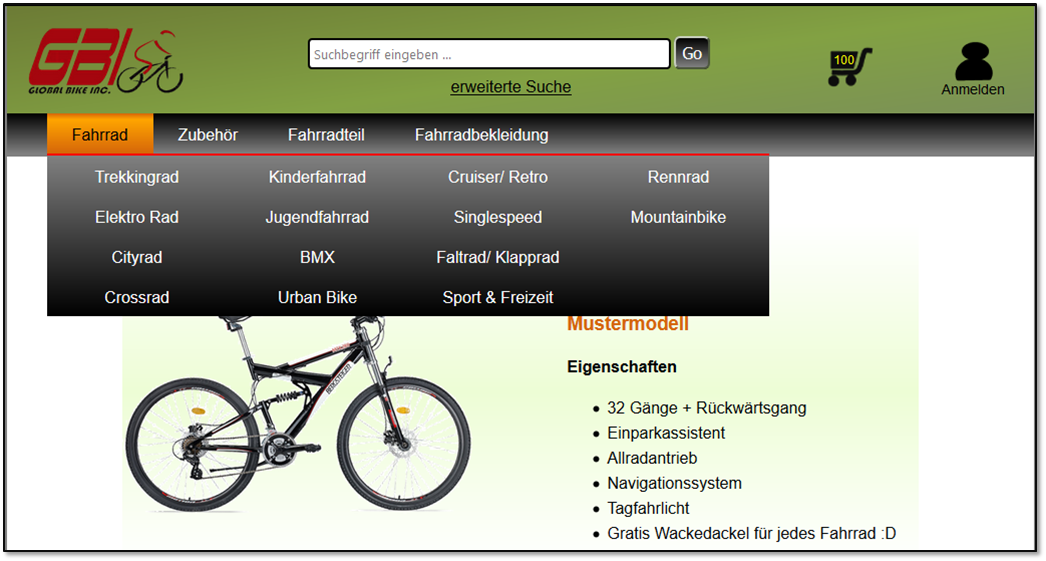
\includegraphics[width=12cm]{Bilder/Abbildung9-DynamischeNaviagtionDesWebshops.png}
\end{center}
\caption{Dynamische Navigation}
\label{Abbildung9-Dynamische Navigation}
\end{figure}

\vfill

\newpage
\begin{center}
	\begin{lstinputlisting}[language=PHP, caption={Auszug aus der Klasse Navigation - Die dynamische Seitennavigation}]
		{Quellcode/navigation.php.inc}
	\end{lstinputlisting}
\end{center}

\newpage
\subsubsection{Arbeitspaket 4: Dynamische Artikelauflistung}

Ein paar Tage später erstellt Herr Schnürer eine dynamische Artikelauflistung. In ihr werden alle Fahrräder einer bestimmten Kategorie aufgelistet. Wählt der Nutzer in der Seitennavigation die Hauptkategorie \glqq{Fahrrad}\grqq{} und anschließend die Unterkategorie \glqq{Cityrad}\grqq{} werden ihm alle \glqq{Cityräder}\grqq{} aufgelistet, wählt er die Unterkategorie \glqq{Mountainbike}\grqq{} werden ihm alle \glqq{Mountainbikes}\grqq{} aufgelistet usw. \textit{Abbildung 19} zeigt die dynamische Artikelauflistung aller \glqq{Cityräder}\grqq{} (Anmerkung: Es wird an dieser Stelle nur ein Cityrad aufgelistet, da sich nur ein Produkt mit der Kategorie \glqq{Cityrad}\grqq{} in der Datenbank befindet. Man müsste nur weitere Cityräder in der Datenbank hinterlegen, damit entsprechend mehr Produkte aufgelistet werden):

\begin{figure}[H]
\begin{center}
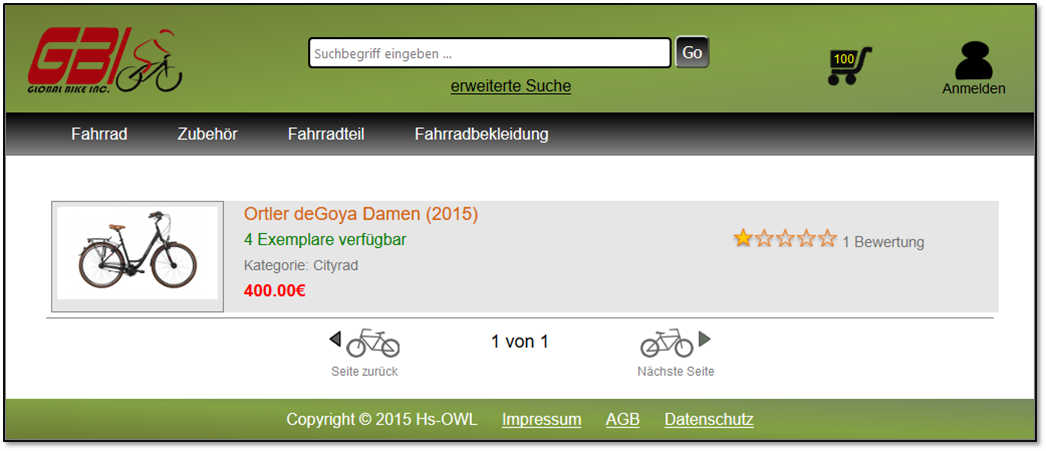
\includegraphics[width=10cm]{Bilder/Abbildung10-DynamischeArtikelauflistungAllerCitybikes.png}
\end{center}
\caption{Dynamische Artikelauflistung aller Cityräder}
\label{Abbildung10-Dynamische Artikelauflistung aller Cityräder}
\end{figure}


\subsubsection{Arbeitspaket 4: Detaillierte dynamische Artikelbeschreibung}

Eine Woche später wird eine detaillierte und dynamische Beschreibung für die Artikel erstellt. Wählt der Nutzer einen Artikel aus, erscheint eine detaillierte Beschreibung dessen. Der oberer Teil ist dabei an die Artikelbeschreibung der Startseite angelehnt und zunähst noch statisch, der untere Teil beschreibt den Artikel näher und ist bereits dynamisch umgesetzt. So erscheint unter der Überschrift \glqq{Artikelbeschreibung}\grqq{} die jeweilige Beschreibung des zuvor ausgewählten Artikels. \textit{Abbildung 20} zeigt eine solche Beschreibung für das Fahrrad \glqq{Ortler deGoya Damen (2015)}\grqq{}:

\begin{figure}[H]
\begin{center}
\fbox{
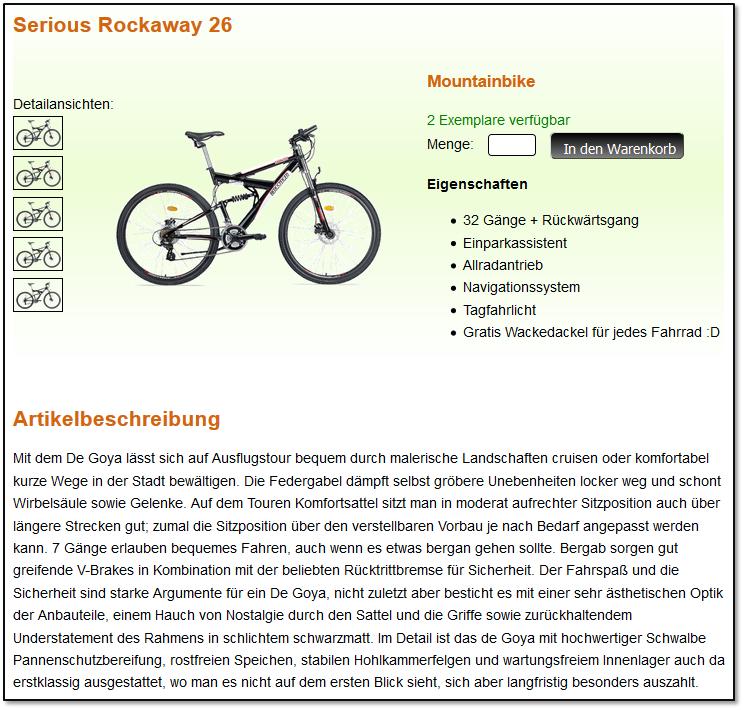
\includegraphics[width=10cm]{Bilder/Abbildung11-DynamischeDetailierteArtikelbeschreibung.png}}
\end{center}
\caption{Detaillierte dynamische Artikelbeschreibung}
\label{Abbildung11-Detaillierte dynamische Artikelbeschreibung}
\end{figure}

Wie bereits erwähnt ist der obere Teil zunähst nur statisch programmiert worden, weshalb die Überschrift noch nicht zum ausgewählten Artikel passt. Der Text \glqq{Artikelbeschreibung}\grqq{} hingegen wird bereits aus der Datenbank geladen.
\\
In den Sommersemesterferien hat Herr Schnürer auch den oberen Teil dieser Seite dynamisch erstellt. Die Produktbilder und Eigenschaften des Artikels werden nun ebenfalls aus der Datenbank geladen. Zudem wird noch ein kleines Extra eingebaut: Klickt der Nutzer eines der Produktbilder an, wird mithilfe eines Java Scripts eine \glqq{Lightbox}\grqq{} aufgerufen. Diese zeigt die Produktbilder in ihrer normalen Auflösung und ermöglicht das einfache Durchklicken der Produktbilder. \textit{Abbildung 21} zeigt den fertigen oberen Teil der Artikelbeschreibung, während \textit{Abbildung 22} die \glqq{Lightbox}\grqq{} veranschaulicht. \textit{Quellcode 3} zeigt, wie dabei vorgegangen wurde:

\begin{figure}[H]
\begin{center}
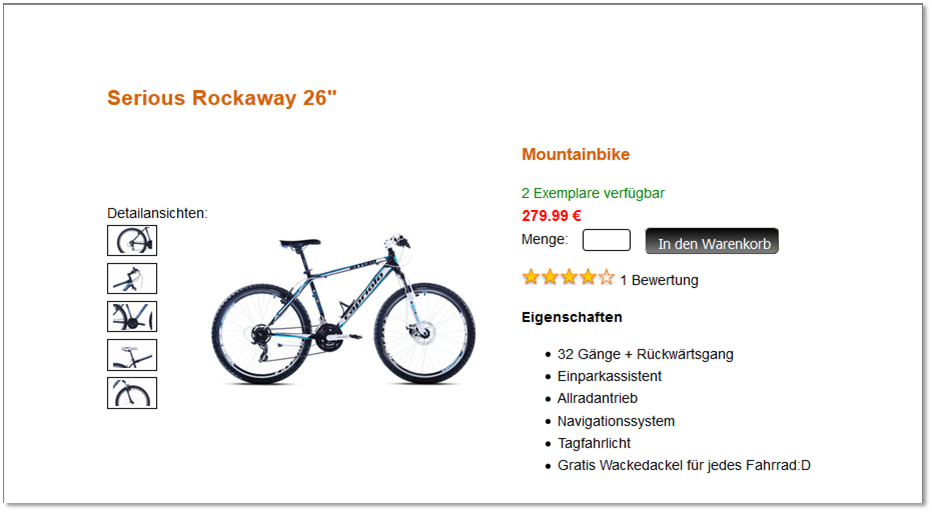
\includegraphics[width=10cm]{Bilder/Abbildung12-DynamischeDetailierteArtikelbeschreibungFertig.png}
\end{center}
\caption{Fertige dynamische Artikelbeschreibung}
\label{Abbildung12-Fertige dynamische Artikelbeschreibung}
\end{figure}

\begin{figure}[H]
\begin{center}
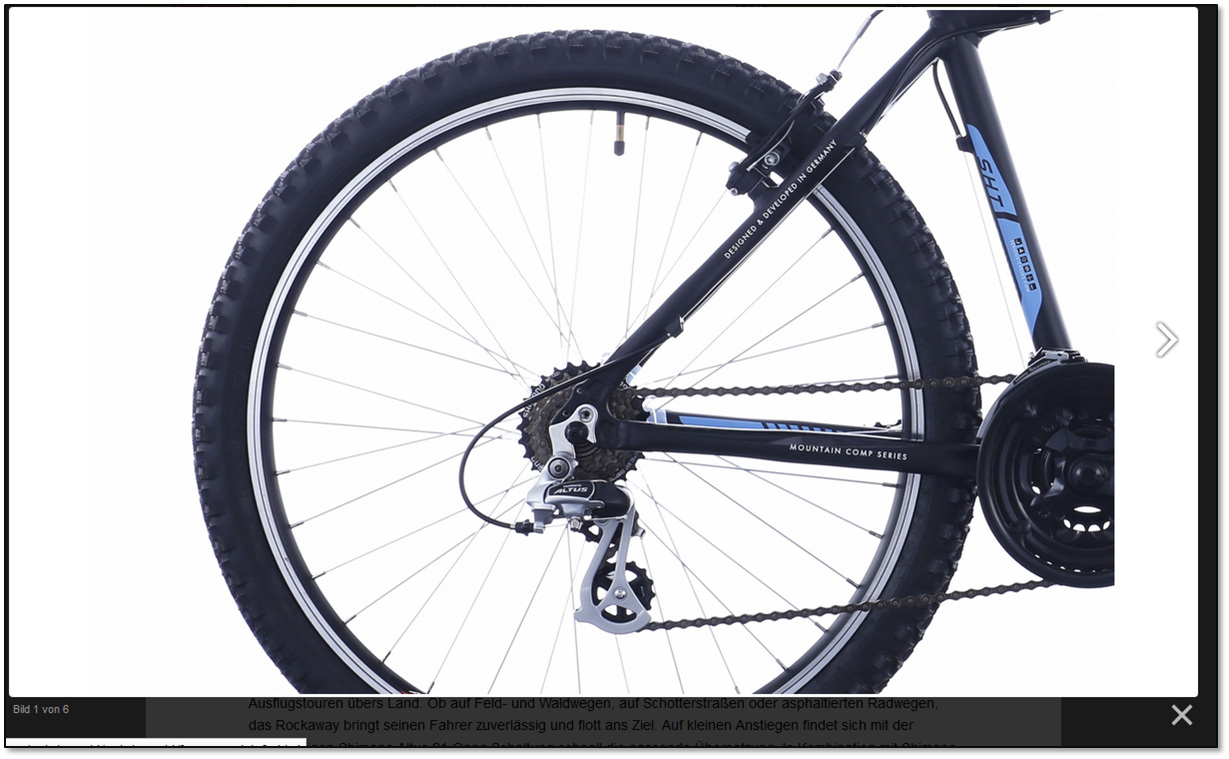
\includegraphics[width=8cm]{Bilder/Abbildung13-Lightbox.png}
\end{center}
\caption{\glqq{Lightbox}\grqq{} zur besseren Darstellung der Produktbilder}
\label{Abbildung13-"Lightbox" zur besseren Darstellung der Produktbilder}
\end{figure}


\begin{center}
	\begin{lstinputlisting}[language=PHP, caption={Auszug aus der Seite Artikel Detailansicht}]
		{Quellcode/ArtikelDetailansicht.php.inc}
	\end{lstinputlisting}
\end{center}


\subsubsection{Arbeitspaket 4: Startseite-Angebot des Tages}

Zum Ende des Projekts wurde die Startseite des Webshops fertiggestellt. Sie zeigt das „Angebot des Tages“ in der oberen Hälfte. In der unteren Hälfte werden die meist angesehenen Artikel des Nutzers angezeigt. \textit{Abbildung 23} zeigt noch einmal die fertige Startseite:

\begin{figure}[H]
\begin{center}
\fbox{
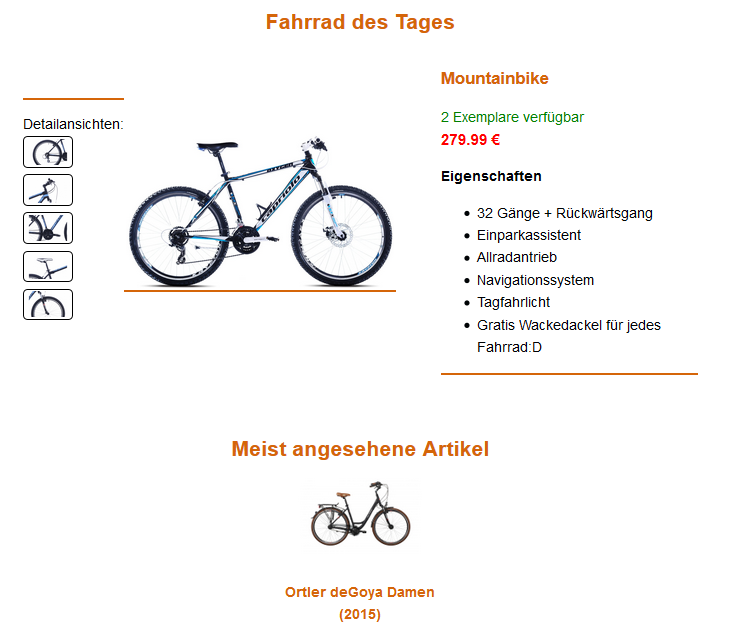
\includegraphics[width=10cm]{Bilder/Abbildung14-StartseiteAngebotDesTages.png}
}
\end{center}
\caption{\glqq{Angebot des Tages}\grqq{}}
\end{figure}


\newpage
\subsection{Arbeitspakete von Herrn Brüntrup}
In diesem Abschnitt wird beschrieben, wie Herr Brüntrup seine Arbeitspakete gelöst hat. Zudem wird in diesem Abschnitt noch beschrieben welche Arbeitspakete wegen Zeitmangel und fehlender Arbeitsbereitschaft zusätzlich noch übernommen wurden.

\subsubsection{Arbeitspaket 5: Die Schnittstellendatenbank}
Die Datenbank stellt die Schnittstelle zwischen dem SAP-System und dem Webshop da. Aus diesem Grund wurde die Datenbankstruktur in der ersten Woche nach der Arbeitspaketverteilung zusammen mit Mitgliedern der SAP-Gruppe entworfen.\\

\textbf{Gründe für die Schnittstellendatenbank}\\
Die Gründe warum die Kommunikation mit einer Schnittstellendatenbank gelöst wurde, wird in den folgenden Sätzen genannt. Der erste Grund war die Verfügbarkeit. Der Webshop sollte auch erreichbar sein, wenn mal keine Verbindung zum SAP-System besteht. Der SAP-Server steht extern bei einer Hochschule in Magdeburg. Es könnte also schon mal dazu kommen, dass das System nicht erreichbar ist. Ein anderer Grund war die Flexibilität. Die Datenhaltung sollte flexibel erweiterbar sein. Soll die Webseite z.B. durch eine 360$^\circ$-Ansicht des Fahrrads erweitert werden, können einfach die benötigten Felder zur Datenbank hinzugefügt werden. Beim SAP-System ist das nur beschränkt möglich. Der Zugriff auf das SAP-System wird mit vordefinierten Funktionen gelöst. Diese Funktionen werden \glqq Business Application Programming Interface (BAPI)\grqq{} genannt. Da die SAP-Gruppe beim SAP-System keine Berechtigungen hat neue BAPIs zu erstellen, wäre somit die Erweiterbarkeit des Webshops sehr eingeschränkt.\\

\textbf{Aufbau der Schnittstellendatenbank}\\
Nun wird der zu Beginn geplante Aufbau der Schnittstellendatenbank erläutert. Die zu Beginn geplante Datenbank bestand aus den Relationen \glqq Kunde\grqq{}, \glqq Bestellungen\grqq{}, \glqq Produkte\grqq{} und \glqq Produktbilder\grqq{}. Die Relation \glqq Kunde\grqq{} enthält die Login-Daten des Kunden sowie dessen Adresse. Die Relation \glqq Bestellungen\grqq{} enthält alle Angaben zur Bestellung. Angaben sind z.B. die Zahlungs- und Versandart sowie der Status der Bestellung. Die vorletzte genannte Relation beinhaltet alle Angaben zu den Produkten, die beim Webshop verkauft werden sollen. Ihr wurde deswegen auch der Name \glqq Produkte\grqq{} gegeben. Die Relation \glqq Produktbilder\grqq{} enthält Pfadangaben, wo auf den Server die Produktbilder abgelegt sind. Da zu einen Produkt mehrere Produktbilder abgelegt werden können, wurde sich auf eine extra Tabelle für die Produktbilder geeinigt.

Eine Relation, die die Produkte einer Bestellung enthält, wurde zunächst vergessen umzusetzen. Das Vergessen der Relation fiel erst auf, als die SAP-Gruppe mit der Umsetzung des Bestellvorgangs bei der SAP-Schnittstelle beginnen wollte. Zur Lösung des Problems fügte die SAP-Gruppe nun nachträglich eine Relation \glqq Bestellprodukte\grqq{} zur Datenbank hinzu. Diese Relation steht in Beziehung mit den Relationen \glqq Bestellungen\grqq{} und \glqq Produkte\grqq{}.

Als Datenbank-Server wurde sich auf MYSQL geeinigt. Dieser Server lässt sich problemlos auf Linux installieren. Es war wichtig, dass die Datenbank unter Linux läuft, da die Server-Gruppe einen Linux-Server aufsetzen wollte. Zudem bietet MYSQL den Vorteil, dass auf eine MYSQL-Datenbank mit der Programmiersprache PHP gut zugegriffen werden kann. Die SAP-Gruppe wollte die Datenbank mit einer selbst geschriebenen JAVA-Anwendung füllen. Auch von JAVA aus kann gut auf eine MYSQL-Datenbank zugegriffen werden. Ein weiterer Grund für die Nutzung der MYSQL-Datenbank war, dass die Softwaresammlung XAMPP einen MYSQL-Server beinhaltet. Die Softwaresammlung XAMPP wurde von der Webshop-Gruppe als Testserver zum Testen der Webseite auf den Hochschulrechnern verwendet. \\
Die \textit{Abbildung 24} zeigt das \glqq Entity-Relationship-Diagramm (ERD)\grqq{}. Dieses Diagramm ist die erste Version der Datenbank, die zusammen mit der SAP-Gruppe entworfen wurde. 

\begin{figure}[H]
	\begin{center}
		\fbox{
			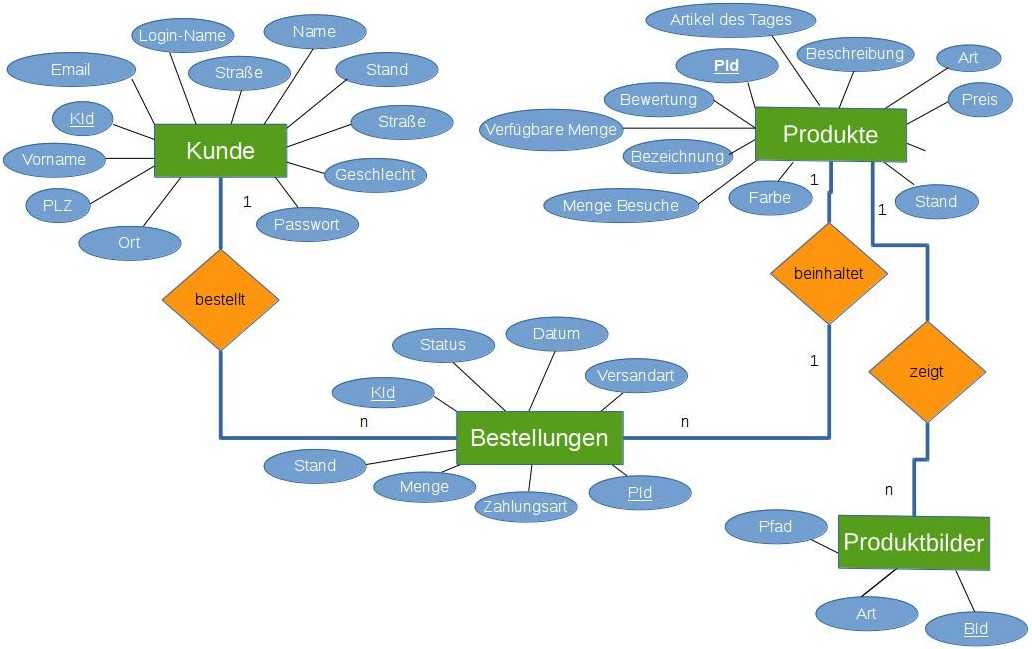
\includegraphics[width=150mm]{Bilder/Abbildung10-erd_alt.jpg}
		}
	\end{center}
	\caption{Erster Datenbankentwurf}
\end{figure}

Da es ursprünglich bemängelt wurde, dass das Projekt noch nicht den für das Modul benötigten Zeitaufwand aufweisen wurde, wurde beschlossen das Arbeitspaket \glqq Bewertung\grqq{} mit einer Kommentarfunktion zu erweitern. Somit sollte der Kunde auch ein Kommentar für seine Bewertung äußern können. Dafür musste die Datenbank etwas angepasst werden. Vorher war einfach ein Attribut \glqq Bewertung\grqq{} in der Relation \glqq Produkte\grqq{} vorzufinden. Um die Kommentare für die Bewertung speichern zu können, wurde die Datenbank um eine Relation \glqq Kommentare\grqq{} erweitert. Diese Relation beinhaltet ein Datenfeld, wo die Bewertung des Kunden (von 1-5 Sterne) gespeichert wird. Ein weiteres Datenfeld der Relation enthält den Bewertungstext. \\
Als mit der Suchfunktion und der Navigation begonnen wurde, fiel schnell auf, dass benötigte Attribute und Tabellen für die Navigation vergessen wurden. Somit wurde eine neue Relation \glqq Produktkategorie\grqq{} zur Datenbank hinzugefügt. Diese Relation steht mit der Relation \glqq Produkte\grqq{} in Beziehung und beinhaltet alle Produktkategorien, die der Webshop anbieten soll. Unter Produktkategorien wird beim Webshop die Festlegung verstanden, ob das Produkt ein Ersatzteil, ein Fahrrad, Zubehör usw. ist. Eine zweite Relation, die mit der Relation Produkte in Beziehung steht, ist die Relation \glqq Bauart\grqq{}. Dieses Relation wird nur verwendet, wenn das Produkt ein Fahrrad ist. In dieser Relation sind alle beim Webshop angebotenen Bauarten aufgelistet. Unter Bauart wird bei diesen Webshop verstanden, ob es sich um ein Mountainbike, Trekkingbike usw. handelt.

Die \textit{Abbildung 25} zeigt die endgültige Struktur der Schnittstellendatenbank mit allen nachträglich hinzugefügten Relationen. 
\begin{figure}[H]
	\begin{center}
		\fbox{
			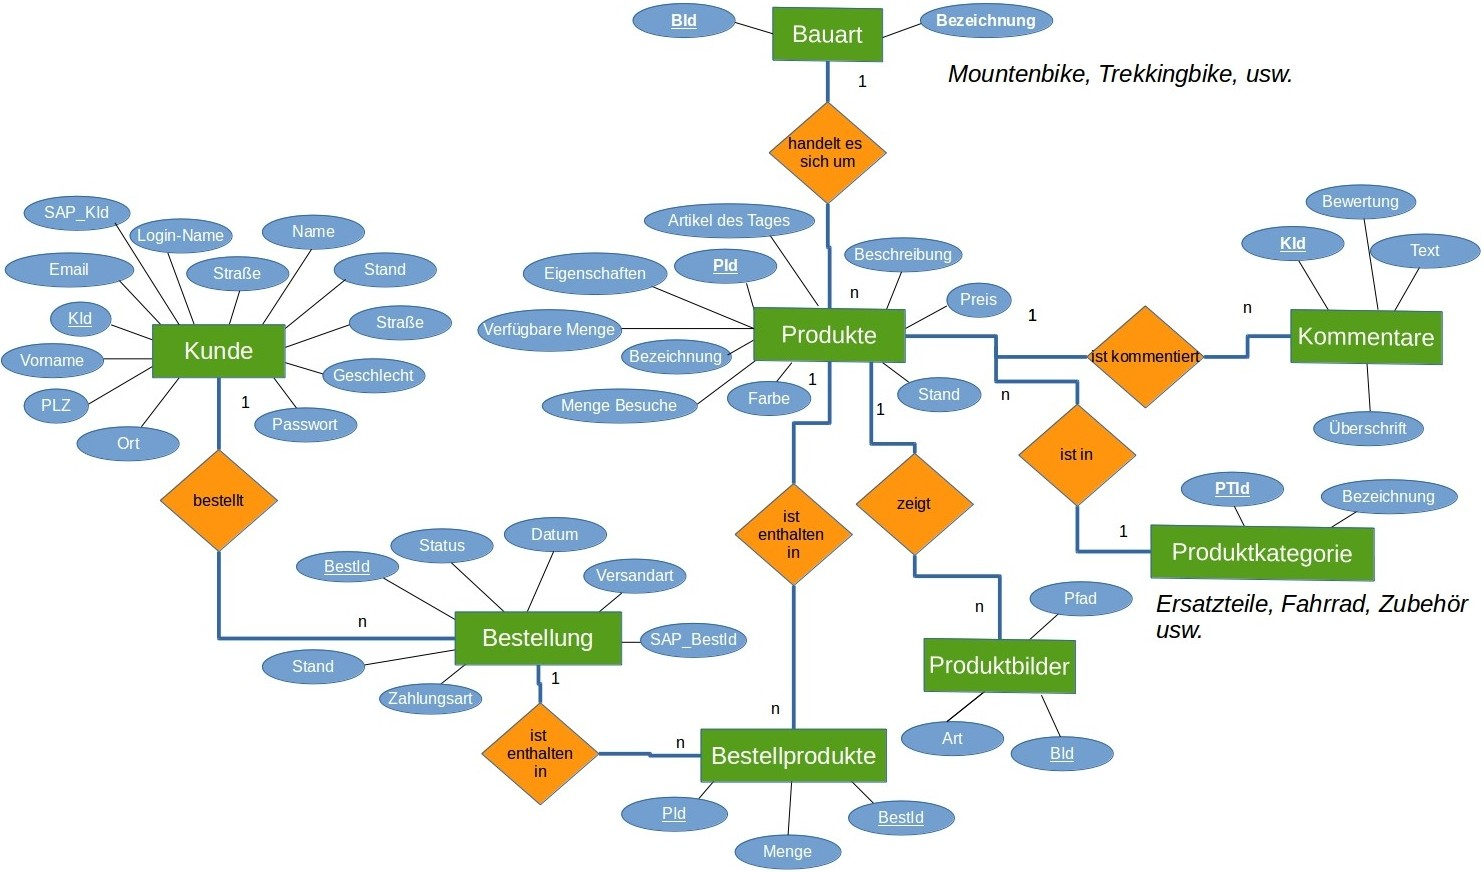
\includegraphics[width=150mm]{Bilder/Abbildung11-erd.jpg}
		}
	\end{center}
	\caption{Endgültiger Datenbankentwurf}
\end{figure}

\textbf{Wahl der PHP-API zum Datenbankzugriff}\\
Um von PHP aus auf eine MYSQL-Datenbank zugreifen zu können, gibt es mehrere Möglichkeiten. In dieser Ausarbeitung werden die Zugriffsmöglichkeiten kurz verglichen und dann erläutert, welche davon für das Projekt benutzt wurde.

Die erste Möglichkeit ist die PHP-API \glqq ext/mysql \grqq{}. Diese API ist veraltet und wird nicht mehr weiterentwickelt. Sie unterstützt noch nicht alle MYSQL 5.1+ Funktionalitäten und ist stellenweise mit neuen PHP-Versionen nicht mehr nutzbar. Diese Erweiterung nutzt den prozeduralen Ansatz. Die nächste Möglichkeit ist die PHP-API \glqq PDO\grqq{}. Diese API unterstützt fast alle Funktionalitäten von MYSQL 5.1+. Sie bietet zudem den Vorteil, dass die API auch zum Zugriff auf andere SQL-basierten Datenbanken genutzt werden kann. Diese API hat einen objektorientierten Aufbau.  Die letzte Zugriffsmöglichkeit bietet die API \glqq ext/mysqli\grqq{}. Sie unterstützt alle MYSQL 5.1+ Funktionalitäten und kann objektorientiert und prozedural programmiert werden.

Die Auswahl fiel auf die API \glqq ext/mysqli\grqq{}. Die Gründe hierfür waren, dass die API alle Funktionalitäten der neusten MYSQL-Version unterstützt, regelmäßig auf die neuesten MYSQL-Funktionen angepasst wird und schon Quellcodes von alten Projekten übernommen werden konnte. Die \textit{Abbildung 26} zeigt die Eigenschaften der drei APIs nochmal in einer Tabelle zusammen gefasst.
\begin{figure}[H]
	\begin{center}
		\fbox{
			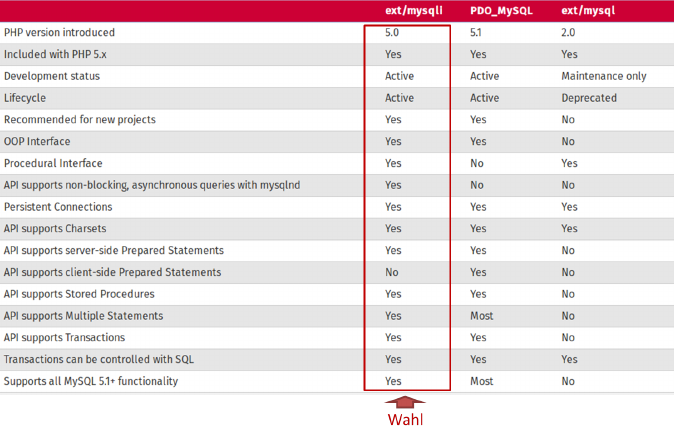
\includegraphics[width=150mm]{Bilder/Abbildung12-mysql_apis.png}
		}
	\end{center}
	\caption{Überblick der PHP-APIs zum Datenbankzugriff}
\end{figure}

\textbf{Die Konfigurationsdatei}\\
Um auf eine MYSQL-Datenbank zugreifen zu können, werden üblicherweise mehrere Zugangsdaten benötigt. Die Zugangsdaten, die mindestens benötigt werden, sind der Datenbankbenutzername, das Passwort zum Benutzername, der Datenbankname und die IP-Adresse des Servers. Damit diese Zugangsdaten nicht bei jeden Datenbankzugriff im Quelltext angegeben werden müssen, wurden diese Angaben in eine Konfigurationsdatei ausgelagert. Wird die Webseiten später mal auf einen anderen Webserver betrieben, so müssen die Datenbankzugangsdaten nur in dieser Datei geändert werden. Die Konfigurationsdatei ist extra gesichert worden, damit sie nicht direkt im Browser geöffnet werden kann. Der Datei wurde als Dateiendung \glqq *.php.inc\grqq{} angehangen. Mit einer bestimmten Zeile in einer Konfigurationsdatei für den Webserver wurde das Öffnen von \glqq *.inc\grqq{}-Dateien den Browser untersagt. Die Konfigurationsdatei trägt den Namen \glqq .htaccess\grqq{} und befindet sich im Home-Vezeichnis der Webseite. Mehr zur \glqq .htaccess\grqq{}-Datei kann im Abschnitt \glqq Sicherheit\grqq{} gelesen werden.

Der \textit{Quellcode 1} zeigt die Konfigurationsdatei des Webshops. In dieser Datei sind die benötigten Datenbankzugangsdaten und die festgelegte Email-Adresse zu lesen, von der alle Bestätigungs-Emails versendet werden sollen. Zudem sind in der Konfigurationsdatei die Bankdaten definiert, die dem Kunden mitgeteilt werden, wenn er als Zahlungsart \glqq Vorkasse\grqq{} ausgewählt hat.
\newpage
\begin{center}
	\begin{lstinputlisting}[language=PHP, caption={Die Konfigurationsdatei}]
		{Quellcode/config.php.inc}
	\end{lstinputlisting}
\end{center}

\textbf{Die Datenbankzugriffsklasse}\\
Beim Webshop wird nicht direkt über die \glqq MYSQLi\grqq{}-API auf die MYSQL-Datenbank zugegriffen. Es wurde für den Datenbankzugriff extra eine Klasse entwickelt, die als Schnittstelle zwischen den Webshop und der \glqq MYSQLi\grqq{}-API fundiert. Diese Klasse bestand schon von alten Projekten und wurde aus folgendem Grund entwickelt. Sie wurde entwickelt, damit nur an einer Stelle das Projekt verändert werden muss, wenn zu einen späteren Zeitpunkt mal ein anderes API verwendet werden soll. Dieses ist z.B. der Fall, wenn zu eine andere Datenbank verwendet werden soll.

\newpage
\subsubsection{Arbeitspaket 6: Registrierungs- und Anmeldungsfenster designen und programmieren}
Dieser Abschnitt beschreibt, wie beim Webshop die Registrierung und Anmeldung umgesetzt wurde. Zudem wird die Umsetzung einer Funktion des Webshops beschrieben, wo der Kunde seine Profildaten ändern kann.\\

\textbf{Der Registrierungsvorgang}\\
Auf dieser Webseite läuft die Registrierung wie in den folgenden Sätzen beschrieben ab. Zunächst tippt der Neukunde die von der Webseite verlangten persönlichen Informationen in ein Formular ein und bestätigt die Eingabe durch einen Klick auf den Bestätigungsbutton. Wenn beim Webbrowser des Neukunden JavaScript nicht deaktiviert ist, überprüft der Webbrowser mit einem JavaScript die Eingabe bevor sie zum Webserver weitergeleitet wird. Die Eingabe wird nur weitergeleitet, wenn diese vom JavaScript aus als gültig anerkannt wurde. Bei ungültiger Eingabe wird auf der Webseite eine Fehlermeldung ausgegeben. Der JavaScript ist keine endgültige Eingabeüberprüfung, dieser dient nur dafür unnötigen Datenverkehr zu minimieren. JavaScript besitzt den Nachteil, dass dieser beim Webbrowser deaktiviert werden kann. Bei deaktivierten JavaScript wird somit die Eingabe unüberprüft an den Webserver weitergeleitet. Somit muss die Eingabe nochmal beim Webserver auf Gültigkeit überprüft werden.  Der Neukunde wird also erst in die Kunden-Tabelle der Datenbank geschrieben, wenn die serverseitig programmierten Überprüffunktionen die Eingabe als gültig angesehen haben. Wurde die Eingabe als ungültig anerkannt, so wird auch bei der serverseitigen Programmierung eine Fehlermeldung auf der Webseite angezeigt. Nachdem der Kunde erfolgreich in der Kundendatenbank angelegt wurde, bekommt der Neukunde eine Bestätigungsmail zu gesendet. Der Neukunde kann sich erst erfolgreich am System anmelden, wenn dieser den in der Email enthaltenden Link ausgeführt hat. 

Das Passwort des Kunden wird nicht in Klartext in die Datenbank gespeichert. Bevor es in die Datenbank geschrieben wird, wird das Passwort mit einen \glqq MD5-Hash-Algorithmus\grqq{} unkenntlich gemacht. Der MD5-Hashwert ist nicht mit einen Schlüssel wieder invertierbar. Er kann zur Speicherung von Passwörtern verwendet werden, da beim \glqq MD5-Hash-Algorithmus\grqq{} der gleiche Input immer den gleichen Output erzeugt. Somit wird beim Login-Check einfach auch das eingegebene Passwort unkenntlich gemacht und verglichen, ob es mit den Wert in der Datenbank übereinstimmt.\\ Die \textit{Abbildung 27} zeigt den Registrierungsvorgang nochmal als BPMN dargestellt.\\

\begin{figure}[H]
	\begin{center}
			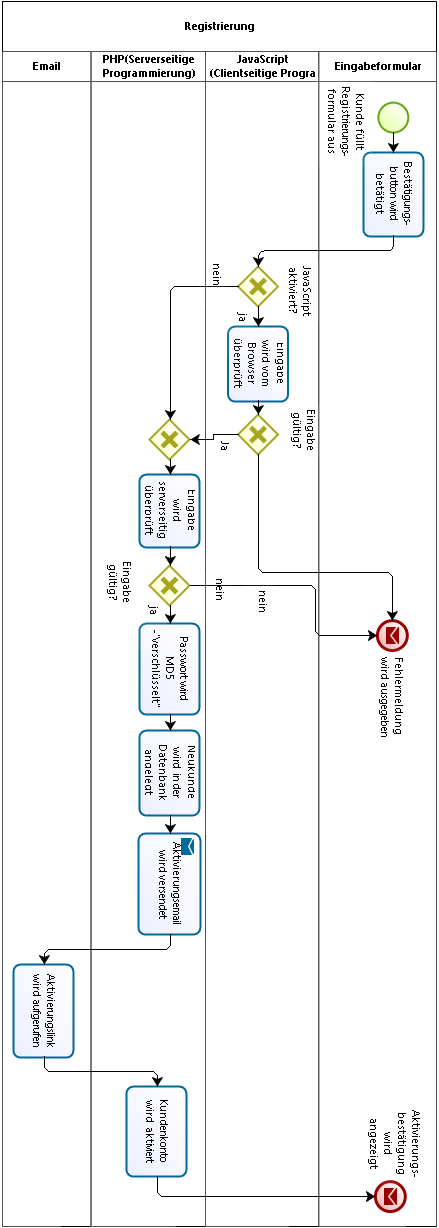
\includegraphics[width=225pt]{Bilder/Abbildung13_Reg_Vorgang.png}
	\end{center}
	\caption{Der Registrierungsvorgang}
	\label{fig:Abbildung 13}
\end{figure}


\textbf{Der Anmeldungsvorgang}\\
Der Anmeldungsvorgang läuft ähnlich wie der Registrierungsvorgang ab. Der Kunde tippt als Benutzernamen seine Email-Adresse und als Passwort das bei der Registrierung angegebene Passwort in das Anmeldeformular ein. Wie bei der Registrierung überprüft ein JavaScript die Eingabe bevor diese an den Server weitergeleitet wird. Die vorherige Überprüfung ist wieder nur bei aktivierten JavaScript im Webbrowser möglich. Deswegen wird die Überprüfung bei der Anmeldung auch nochmal vom Server überprüft. Hat der Kunde eine gültige Eingabe getätigt, so wird die Email-Adresse und das Passwort mit den Datensätzen in der Kunden-Tabelle der Datenbank verglichen. Um den Vergleich ausführen zu können wird bei der Anmeldung auch das Passwort durch den  \glqq MD5-Hash-Algorithmus\grqq{} unkenntlich gemacht. Wurde in der Tabelle ein Datensatz gefunden, wo Email-Adresse und Passwort übereinstimmen, so wird der Kunde eingeloggt. Wurde keine Übereinstimmung gefunden, so wird auf der Webseite eine Fehlermeldung ausgegeben.\\ 
Der Einlogvorgang wurde wie folgt umgesetzt. Die Anmelde-Email-Adresse wird in einer SESSION-Variable gespeichert. Der SESSION-Variable wurde der Name \glqq \$\_SESSION[ 'angemeldet' ]\grqq{} gegeben. An Hand dieser Variable erkennt der Webshop, ob der Kunde angemeldet ist oder nicht. Wurde die Variable angelegt und enthält einen Wert, so wird dieses als angemeldet interpretiert. Die Abmeldung erfolgt einfach durch das Löschen dieser Variable. Eine SESSION-Variable behält die enthaltenden Daten über mehrere Seitenaufrufe. Wenn nicht mehr auf die Variable zugegriffen wird, werden die Daten dieser Variable automatisch nach einer bestimmten Zeit gelöscht. Ob der Kunde angemeldet ist, muss in einer SESSION-Variable zwischengespeichert werden, da das HTTP-Protokoll verbindungslos ist. Es wird also jede HTTP-Anfrage isoliert betrachtet. Ohne die SESSION-Variable könnte sich somit der Webserver nicht merken, dass der Kunde angemeldet ist. Einer Session wird in PHP eine eindeutige \glqq SESSION-ID\grqq{} zugeordnet. Diese SESSION-ID wird entweder als Cookie im Browser abgespeichert oder immer der Seiten-URL mit übergeben. Wird die SESSION-ID in einem Cookie im Browser abgespeichert, so wird dieser beim Schließen des Browsers gelöscht. Die Daten, die in der SESSION-Variable abgespeichert sind, werden auf der Serverseite zwischengespeichert und nicht im Browser. Die SESSION-ID wird von Browser bei jeder Anfrage an den Server weitergeleitet. An Hand dieser SESSION-ID kann der Server die SESSION-Variable zu den entsprechenden Browser zuordnen.\\

\textbf{Die clientseitige Überprüfung}\\
Wenn JavaScript aktiviert ist, werden, wie oben schon erwähnt, die Formulareingaben zuvor im Browser überprüft. Dafür wird beim Formular den Attribut \glqq onsubmit\grqq{} eine JavaScript-Funktion übergeben. Die Formulareingabe wird hierbei nur an den Server weitergeleitet, wenn diese Methode als Rückgabewert \glqq true\grqq{} zurückgibt. Die JavaScript-Funktion überprüft bei der Eingabe, ob überhaupt ein Text in die Textfelder eingegeben wurde und die Eingabe gültig ist. Zum Beispiel darf eine Postleitzahl nur aus 5 Ziffern bestehen. Die clientseitige Programmierung findet bei der Anmeldung in der Datei \glqq /Funktions/JS/anmeldung.js\grqq{} und bei der Registierung in der Datei \glqq /Funktions/JS/registrierung.js\grqq{} statt.

\newpage
\begin{center}
	\begin{lstinputlisting}[language=HTML, caption={Login-Formular (vereinfacht)}]
		{Quellcode/login-formular.php.inc}
	\end{lstinputlisting}
\end{center}

Der \textit{Quellcode 2} zeigt in vereinfachter Version das Login-Formular. Beim \glqq form\grqq{}-Tag kann das \glqq onsubmit\grqq{}-Attribut gefunden werden. Dieses Attribut startet beim Klick auf den Submit-Button die enthaltende JavaScript-Funktion. Das Attribut lässt nur die Durchführung des Submits zu, wenn die JavaScript-Funktion als Rückgabewert den Wert \glqq true\grqq{} zurückliefert.

Um unnötigen Quelltext zu umgehen, wurde ein Teil des Eingabeüberprüfungsquellcode in eine andere JavaScript-Datei ausgelagert. Der ausgelagerte Quellcode wird bei jeden Formular benötigt. Dieser Quellcode überprüft, ob alle Pflichtfelder ausgefüllt sind. Die ausgelagerte Funktion trägt den Namen \glqq sindAlleFelderAusgefuellt\grqq{} und befindet sich in der Datei \glqq /Funktions/JS/vorcheck\_std\_funktionen.js\grqq{}. Der Funktion werden beim Aufruf drei Parameter übergeben. Der erste Parameter erhält ein Array. Dieses Array enthält die Feldnamen der Textfelder, wovon die Eingabe überprüft werden soll. Der zweite Parameter enthält wiederum ein Array. Dieses Array enthält die Meldungswörter, die in der Fehlermeldung für das jeweilige Textfeld eingesetzt werden sollen. Die Meldungswörter werden in die Fehlermeldung eingesetzt, wenn das Textfeld nicht gefüllt ist. Beim letzten Parameter wird der Name des Formulars angeben, worauf sich die Textfelder befinden. Sind nicht alle Felder ausgefüllt, erstellt die Funktion eine Fehlermeldung und gibt diese als Rückgabewert aus.\\
In die Auslagerungsdatei wurden zudem Funktionen zur Überprüfung der Email-Adresse oder ob die Eingabe eine Zahl ist abgelegt. Die Funktionen in den Dateien \glqq /Funktions/JS/anmeldung.js\grqq{} und  
\glqq /Funktions/JS/registrierung.js\grqq{} rufen die ausgegliederten Funktionen auf und führen noch eine genauere Überprüfung durch. Die Funktionen testen zum Beispiel, ob das Passwort mit der Passwortwiederholung übereinstimmt.\\

\textbf{Serverseitige Programmierung}\\
Wie bei der clientseitigen Programmierung wurde auch bei der serverseitigen Programmierung die Methode zur Überprüfung ob alle Pflichtfelder ausgefüllt sind ausgelagert. Bei der serverseitigen Programmierung wurde hierfür die Technik der Vererbung genutzt. Serverseitig wurde der Webshop objektorientiert programmiert. Für die zuvor genannte Methode wurde die Klasse \glqq EingabeCheckGrundlegend\grqq{} erstellt. Diese Klasse wurde an alle anderen Klassen vererbt, die Formulareingaben entgegen nehmen müssen. Für die Registrierung, Anmeldung und Änderung des Kundenprofils ist die Klasse \glqq Kunde\grqq{} entwickelt worden. Sie enthält Methoden, mit der die Formulareingabe überprüft, ein neuer Kunde angelegt, ein Kunde verwaltet und die Anmeldung durchgeführt werden kann.\\
Instanziiert wird die Klasse durch Skripte des Ordners \glqq /Funktions/PHP\grqq{}. Registriert sich ein neuer Kunde am Webshop, so wird von den Registierungsformular der Skript \glqq registrierung\_durchfuehren.php.inc\grqq{} des zuvor genannten Ordners aufgerufen. Dieser Skript instanziiert die Klasse \glqq Kunde\grqq{}, überprüft die Formaulareingabe und legt bei gültiger Eingabe den Kunden an. Zur Überprüfung der Eingabe und zum Anlegen des Kunden ruft der Skript die benötigten Methoden der Klasse \glqq Kunde\grqq{} auf.\\
Weitere Skripte, die mit der Klasse \glqq Kunde\grqq{} arbeiten, sind zum Beispiel die Skripte \glqq anmeldung\_durchfuehren.php.inc\grqq{}, \glqq kunde\_aktivieren.php.inc\grqq{} und \glqq kunde\_aendern.php.inc\grqq{}. Der erste der Skript der Liste ist für die Anmeldung des Kunden zuständig, der zweite aktiviert den Kunden, wenn der Aktivierungslink der Aktivierungsemail angeklickt wurde und der letzte Skript ist für das Ändern der Anschrift oder Benutzerkennung des Kunden zuständig.\\
Die Klasse \glqq Kunde\grqq{} legt alle Daten in der Datenbank ab. Wird z.B. die Instanzmethode \glqq get\_vorname\_from\_kid(\$kid)\grqq{} aufgerufen, so fragt die Methode über einen Datenbank-Select den Vornamen des Kunden von der Datenbank ab. Das Java-Schnittstellenprogramm der SAP-Gruppe lauscht die ganze Zeit, ob sich etwas an der Datenbank ändert. Kam es zu einer Änderung in der Datenbank, so wird die Änderung im SAP-System eingetragen.\\

\textbf{Der Loginbereich im Header}\\
Der Loginbereich im Header wurde mit einen sogenannten \glqq Flyout\grqq{} umgesetzt (siehe \textit{Abbildung 28}). Ein Flyout blendet ein Fenster auf der Webseite ein, wenn über ein bestimmtes Symbol mit der Maus gefahren wird. Der Loginbereich bei der Webseite wird also erst angezeigt, wenn sich die Maus auf den Anmeldesymbol befindet. 

\begin{figure}[H]
	\begin{center}
			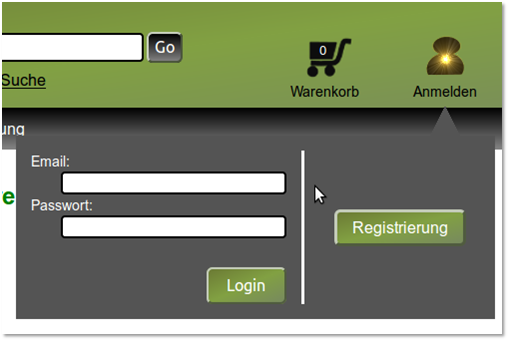
\includegraphics[width=75mm]{Bilder/Abbildung14_Loginbereich.png}
	\end{center}
	\caption{Flyout: Loginbereich}
\end{figure}

Die Besonderheit bei den Flyout des Webshops ist, dass es auch bei deaktivierten JavaScript funktioniert.  Das Flyout wurde mit den in CSS 2.0 eingeführten \glqq Kindselektor\grqq{} umgesetzt. Mit diesen \glqq Kindselektor\grqq{} ist es eingeschränlt möglich mit CSS eventbasiert zu programmieren. Um diese CSS-Funktion nutzen zu können, muss aber folgende Bedingung erfüllt sein: Das Fenster, dass angezeigt werden soll muss ein Kindelement des Elements sein, welches das Ereignis auslöst. Die Syntax des \glqq Kindselektors\grqq{} sieht wie im \textit{Quellcode 3} zeigt aus. Am Anfang steht die Bedingung, die am Elternelement erfüllt sein muss. Beim Webshop wäre es die Bedingung, dass die Maus sich auf den Anmeldesymbol befinden soll. Diese Bedingung sieht in CSS geschrieben folgendermaßen aus: \glqq .accountCell:hover\grqq{}. Darauf folgt ein \glqq >\grqq{}-Zeichen. Dieses Zeichen legt fest, dass bei erfüllter Bedingung nicht die Style-Anweisung des Elternelements verändert werden soll, sondern die Style-Anweisung eines Kindelementes. Nachfolgend wird das Kindelement angegeben, wo die Style-Anweisung geändert werden soll. Der letzte Teil der Style-Anweisung legt das neue Aussehen des Kindelements fest. Beim Webshop wird hier festgelegt, dass das Kindelement sichtbar werden soll. Ein Paar Zeilen vorher definiert eine Anweisung, dass das Kindelement unsichtbar sein soll. Bei gültiger Bedingung wird diese Anweisung einfach von der eben genannten Anweisung überschrieben.

\begin{center}
	\begin{lstinputlisting}[language=CSS, caption={Loginbereich: Umsetzung des Flyouts mit CSS 2.0}]
		{Quellcode/flylayout.css}
	\end{lstinputlisting}
\end{center}

\textbf{Kundenprofil ändern}\\
Hat sich eine Kunde angemeldet, so bietet der Webshop ihn die Möglichkeit die bestehenden Login-Daten und die persönliche Anschrift zu ändern. Erreicht können die Formulare zur Änderung der Daten über ein Flyout. Wenn der Kunde angemeldet ist wird das Flyout unter den Anmeldesymbol zu einem Menü geändert (siehe \textit{Abbildung 29}).
\begin{figure}[H]
	\begin{center}
			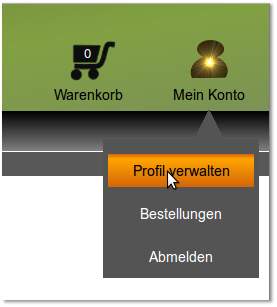
\includegraphics[width=55mm]{Bilder/Abbildung15_Menue_Profil_aendern.png}
	\end{center}
	\caption{Flyout: Kunde angemeldet}
\end{figure}
Bei diesem Menü muss der Eintrag \glqq Profil verwalten\grqq{} gewählt werden, um die bestehenden Login-Daten und die persönliche Anschrift ändern zu können. Nach der Anwahl des Eintrags bekommt der Kunde die in der \textit{Abbildung 30} gezeigte Seite zu sehen.
\begin{figure}[H]
	\begin{center}
			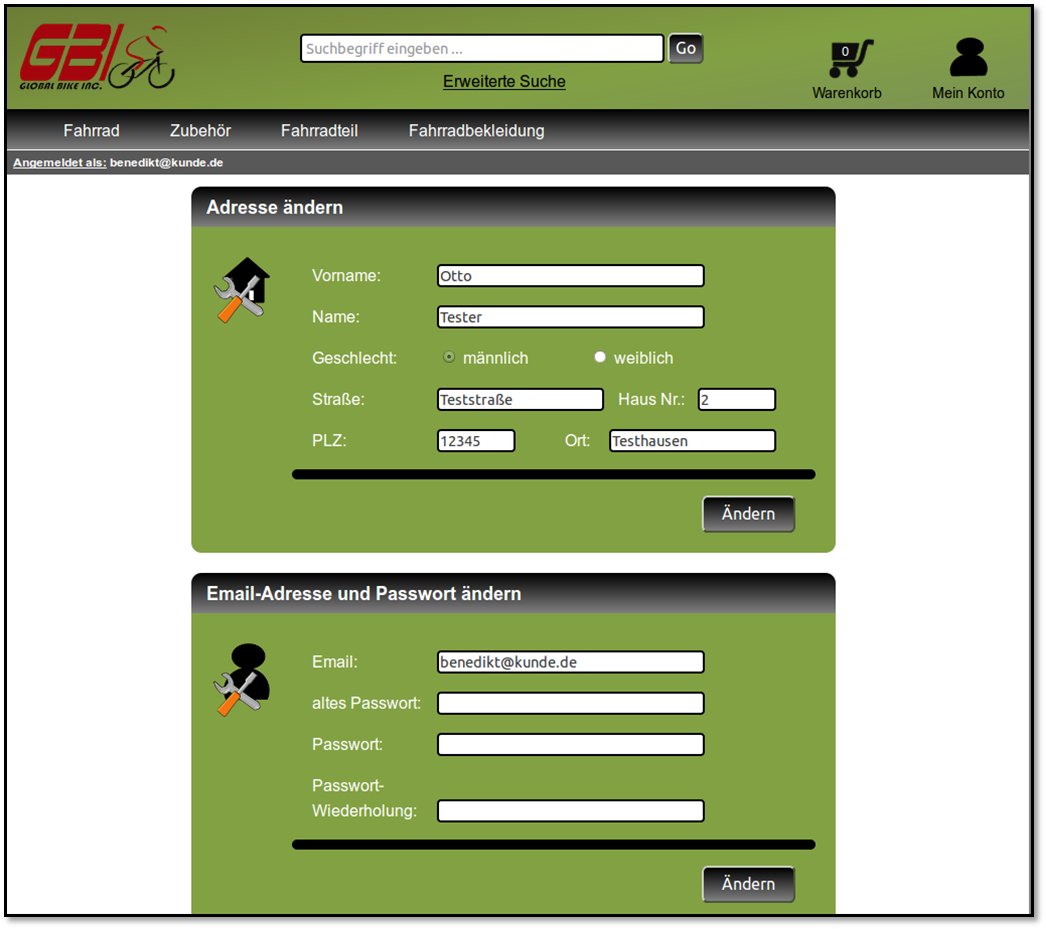
\includegraphics[width=130mm]{Bilder/formulare_profil_aendern.png}
	\end{center}
	\caption{Formulare Kundenprofil ändern}
\end{figure}
Die Änderung des Kundenprofils wurde mit Hilfe von zwei Formularen umgesetzt. Das erste Formular ändert die Anschrift des Kunden und das andere die Logindaten. Der Vorteil dieser zwei Formulare ist, dass somit die Seite übersichtlicher gestaltet ist und meist der Kunde  nur die Adresse ändert, wenn er umgezogen ist. Häufiger wird es wahrscheinlich vorkommen, dass der Kunde das Loginpasswort ändert. Durch die Trennung der Adresse und der Logindaten werden bei Änderung des Passworts nur das neue Passwort und die Login-Email-Adresse an den Server übertragen und neu in die Datenbank geschrieben. Somit werden so wenig wie möglich unnötige Daten zum Server übertragen.\\
Technisch umgesetzt wurde der Vorgang wie beim Registrierungsvorgang. Wenn JavaScript aktiviert ist, überprüft die JavaScript-Funktion \glqq vorcheckEingabeEmailPasswort()\grqq{} oder \glqq vorcheckEingabeAdresse()\grqq{} browserseitig die Eingabe. Die aufgerufene Funktion ist abhängig von welchen Formular der Submit-Button geklickt wurde. Diese Funktionen sind in der Datei \glqq /Funktions/JS/ \\ vorcheck\_profil\_aendern.js\grqq{} vorzufinden. War die Überprüfung nicht erfolgreich, wird wieder eine Fehlermeldung auf den entsprechenden Formular ausgegeben. War die Überprüfung erfolgreich, wird aus den bekannten Gründen diese nochmal auf dem Server durchgeführt. War die serverseitige Überprüfung erfolgreich, ruft die Funktionsdatei \glqq /Funktions/PHP/kunde\_aendern.php.inc\grqq{} die entsprechende Änderungsmethode der Klasse \glqq Kunde\grqq{} auf und übergibt der Methode als Parameter die Formulareingabe. Diese Methode ändert die entsprechenden Werte in der Datenbank mit Hilfe einer Update-SQL-Anweisung. Wurde die Änderung erfolgreich ausgeführt, wird der Kunde über eine Informationsbox darüber informiert.

\subsubsection{Arbeitspaket 7: Entwickeln einer Suchfunktion}
Dieser Abschnitt beschreibt, wie die Suche beim Projekt umgesetzt wurde. Der Webshop hat eine \glqq normale\grqq{} und eine \glqq erweiterte\grqq{} Suche erhalten. Zudem wurde eine abstrakte Klasse entworfen, die Methoden für die Auflistung der Suchergebnisse bietet. Dieses Klasse wurde an die Klasse für die Suche vererbt und konnte ebenso von Herrn Schnürer für die Auflistung der über die Navigation gefundenen Produkte einer Kategorie verwendet werden.\\

\textbf{Suchwortvervollständigung}\\
Die Suchfunktion wurde beim Webshop mit einer Suchwortvervollständigung ausgerüstet. Diese Vervollständigungsfunktion ist mit Ajax programmiert worden. Mit Ajax kann der Browser über JavaScript, während eine Webseite geöffnet ist, Anfragen an den Server senden und die Antwort des Servers entgegen nehmen. Für den Webserver sind diese Anfragen wie ganz normale Seitenaufrufe. Will der Browser Parameter zur Anfrage hinzufügen, werden diese über \glqq GET\grqq{} übermittelt. Dieses heißt, dass die Parameter an die Adressenzeile angehängt werden.\\
Programmiert wurde die Suchwortvervollständigung, wie es in den folgenden Zeilen beschrieben wird. Beim Textfeld ruft das Attribut \glqq onkeyup\grqq{} eine JavaScript-Funktion der Datei \glqq /Funktions/JS/suche.js\grqq{} auf. Diese Funktion sendet mit AJAX eine Anfrage an den Server. Bei dieser Anfrage fragt der Browser den Server an, ob zu der Eingabe etwas in der Datenbank gefunden werden kann. Mit der Zeile \glqq html2.onreadystatechange = autovervollstaendigung\_normale\_suche\_result\_erweiterte\_suche;\grqq{} wird die Funktion festgelegt, die der JavaScript aufrufen soll, falls der Server antwortet. Diese Funktion nimmt den Rückgabewert des Servers entgegen und gibt diesen in einen DIV auf der Webseite aus.  Der Rückgabewert ist mit Hyperlinks versehen. Diese Hyperlinks sorgen dafür, dass bei Anwahl eines der Rückgabewerte das Suchtextfeld mit diesen Wert gefüllt wird und somit das Suchwort vervollständigt wurde. Die serverseitige Umsetzung der Suchwortvervollständigung findet in der Datei \glqq /Funktions/PHP/ajax\_autovervollstaendigung\_suche.php\grqq{} statt. Diese Datei instanziiert eine für die Suche entwickelte Klasse, wenn beim Aufruf der Datei ein Suchwort via GET-Parameter übergeben wurde. Die entwickelte Klasse trägt den Namen  \glqq Suche\grqq{}. Nach der Instanziierung ruft die Datei eine Suchmethode der Klasse auf und gibt das Suchergebnis mit den Befehl \glqq echo\grqq{} aus. Der Suchmethode wird als Parameter der Suchbegriff übergeben. Die aufgerufene Methode ist abhänig von der Suchfunktion. Wurde die Anfrage von der \glqq normalen\grqq{} Suchfunkton gesendet wird die Methode \glqq normale\_suche\_autovervollstaendigung()\grqq{} aufgerufen. Ist der Absender der Anfrage die \glqq erweiterte\grqq{} Suche, so wird die Methode \glqq erweiterte\_suche\_autovervollstaendigung()\grqq{} aufgerufen. Die Ausgabe der Datei wird später von den JavaScript als den eben genannten Rückgabewert entgegengenommen. \\

\newpage
\textbf{Die eigentliche Suchfunktion}\\
Beim Webshop wurden zwei Suchfunktionen implementiert. Eine \glqq normale\grqq{} Suche im Header der Webseite und eine \glqq erweiterte\grqq{} Suche. Bei der erweiterten Suche (siehe \textit{Abbildung 34}) kann der Kunde die Suche noch genauer spezifizieren. Der Kunde kann z.B. Angaben machen, um was für eine Bauart von Fahrrad es sich handeln soll (Mountainbike, Rennrad,...). Der Suchvorgang läuft bei beiden Suchfunktionen gleich ab. Wird der Submit-Button geklickt, wird zunächst erst über JavaScript überprüft, ob die Eingabe gültig ist. Wie schon beim letzten Arbeitspaket erläutert, dient die browserseitige Überprüfung mit JavaScript nur zur Einsparung von unnötigen Datenverkehr zwischen Server und Browser. Aus den von letzten Arbeitspaket bekanntem Grund wird die Eingabeüberprüfung nochmal mit PHP durchgeführt. War die Eingabeüberprüfung mit PHP erfolgreich, wird die für die Suchfunktion entsprechende Methode der Klasse \glqq Suche\grqq{} aufgerufen. Die Suche wird innerhalb der Methoden rein in SQL umgesetzt. Bei SQL-Datenbanken ist die Suche praktisch schon fertig erhältlich. Der Programmierer muss nur einen entsprechende Abfrage formulieren und bekommt von der Datenbank die entsprechenden Rückgabewerte. Wird bei SQL der \glqq like\grqq{}-Operator verwendet, so unterstützt SQL auch Platzhalter für mehrere Zeichen. Diese wurden bei den Suchfunktionen benutzt, um festzulegen, dass hinter und vor den Suchbegriff noch andere Zeichen stehen dürfen.

\begin{figure}[H]
	\begin{center}
			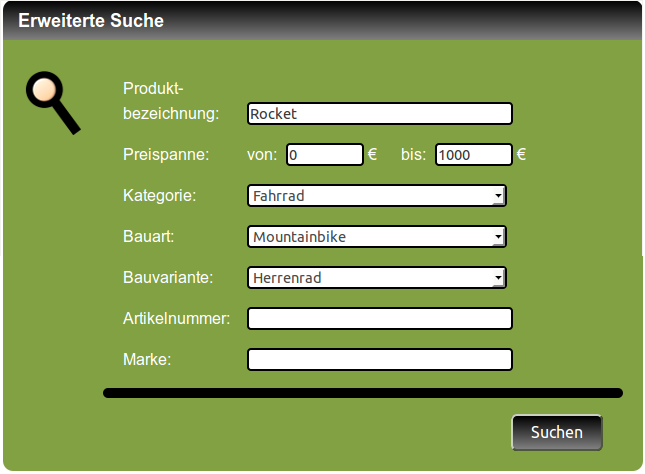
\includegraphics[width=115mm]{Bilder/erweiterte_suche.png}
	\end{center}
	\caption{Formular: Erweiterte Suche}
\end{figure}

\textbf{Anzeige der Suchergebnisse}\\
Bei der Anzeige der Suchergebnisse wurde versucht den Quelltext so zu programmieren, dass Herr Schnürer so viel wie möglich für die Navigation übernehmen konnte. Es wurde somit versucht, so viel wie möglich in eine Klasse auszulagern. Diese Klasse wurde so entwickelt, dass diese an die Navigations- und Suche-Klasse vererbt werden konnte. Die vererbten Methoden mussten also nur einmal programmiert werden. Der Klasse wurde der Name \glqq Artikelauflistung\grqq{} gegeben. Sie ist in der Datei \glqq /Classes/artikel.php.inc\grqq{} zu finden. Die Klasse enthält unter anderem eine Methode, die als Parameter den direkten Rückgabewert des Datenbankservers auf eine SQL-Anweisung entgegennimmt und aus den Rückgabewert eine übersichtliche Liste der Produkte erstellt. Die Liste zeigt den Produktnamen, die vorhandenen Exemplare, die Produkt-Kategorie, den Preis und die Bewertung des Produktes an. Zudem ist ein Bild des Produktes zu sehen. Damit die Methode eine Leiste zur Seitenwahl am Ende der Webseite anzeigen kann, müssen der Methode noch weitere Parameter übergeben werden. Es wird in einem Parameter übergeben, welche Seitennummer aktuell aufgerufen ist. Ein anderer Parameter nimmt entgegen, wie viele Seiten insgesamt zum Suchergebnis gefunden wurden. \\
Die Methode kann nur den Datenbankrückgabewert verarbeiten, wenn dieser die festgelegten Feldnamen enthält. Da bei der Navigation und der Suche die SQL-Anweisung fast gleich sind, wurde der gleiche Teil in eine Methode ausgelagert. Diese Methode gibt somit den vorderen Teil der SQL-Anweisung als Rückgabe aus. Für die Suche und die Navigation muss in der entsprechenden Klasse also nur noch der Rückgabewert dieser Methode durch den \glqq WHERE-Teil \grqq{} der Anfrage ergänzt werden.\\
Die \textit{Abbildung 32} zeigt wie ein Suchergebnis des Webshops aussieht. Beim gezeigten Suchergebnis wurde nach Fahrrädern im Preisbereich zwischen 250 und 400 € gesucht.

\begin{figure}[H]
	\begin{center}
			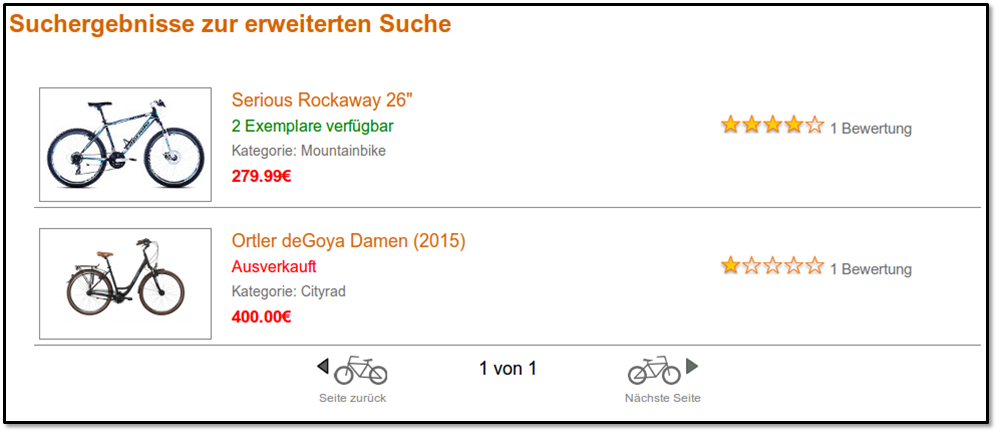
\includegraphics[width=130mm]{Bilder/suchergebnis.png}
	\end{center}
	\caption{Suchergebnis}
\end{figure}

\subsubsection{Zum Teil übernommenes Arbeitspaket: Warenkorb}
Auf Grund von mehreren Fehlstunden des Gruppenmitglieds Raphael Gregarek war es beim Projektverlauf zu größeren zeitlichen Rückständen beim Arbeitspaket \glqq Warenkorb\grqq{} gekommen. Da die Arbeitspakete von Benedikt Brüntrup schon weitgehend fertig waren, wurde somit die restlichen Aufgaben des Arbeitspaketes \glqq Warenkorb\grqq{} von Herrn Brüntrup übernommen. Die Einarbeitungszeit in den bestehenden Quellcode war recht kurz, da dieser schon von Hilfestellungsarbeiten bekannt war. In den folgenden Zeilen wird beschrieben welche Funktionen des Arbeitspaketes Herr Brüntrup umgesetzt hat.\\

\newpage
\textbf{Eingabeüberprüfung}\\
Wie bei den anderen Formularen wurde auch beim Warenkorb eine Eingabeüberprüfung programmiert. Diese wurde clientseitig in der Datei \glqq /Funktions/JS/vorcheck\_warenkorb.js\grqq{} und serverseitig in der Datei \glqq /Funktions/PHP/warenkorb.php.inc\grqq{} umgesetzt. Die Überprüfung wurde, wie bei den anderen Formularen umgesetzt und wird deswegen nicht weiter in dieser Ausarbeitung erläutert. Die Eingabeüberprüfung überprüft, ob überhaupt eine Menge angegeben wurde und ob diese im gültigen Bereich liegt. Es können somit keine negative Mengen und auch nicht mehr Produkte als auf Lager sind bestellt werden. Zudem wird als Wert nur eine ganze Zahl unterstützt. Die \textit{Abbildung 33} zeigt die Fehlermeldung der Eingabeüberprüfung, wenn der Kunde mehr Artikel bestellen will, als auf Lager sind.\\

\begin{figure}[H]
	\begin{center}
			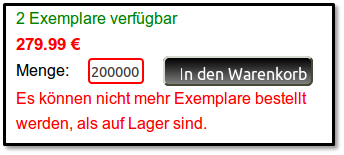
\includegraphics[width=55mm]{Bilder/warenkorb_eingabepruefung.png}
	\end{center}
	\caption{Eingabeüberprüfung Warenkorb}
\end{figure}

\textbf{Warenkorbübersichtsseite}\\
Bei der Warenkorbübersichtsseite handelt es sich um eine Seite, wo der Kunde den Warenkorbinhalt genaustens aufgelistet bekommt. Auf dieser Seite kann der Kunde die Bestellmenge nachträglich verändern oder das Produkt ganz aus dem Warenkorb entfernen.
Zur Umsetzung dieser Seite wurden die von Herrn Gregarek schon entwickelten Klassen um Methoden erweitert. Herr Gregarek hatte bis zum Zeitpunkt der Erstellung der Warenkorbübersichtsseite schon ein Flyouts im Header der Webseite entwickelt, welches den Kunden übersichtlich die Artikel anzeigt, die sich im Warenkorb befinden. Das Flyout dient nur als Schnellübersicht und bietet keine Funktionen, um den Inhalt des Warenkorbs bearbeiten zu können. Die \textit{Abbildung 34} zeigt die Warenkorbübersichtsseite.

\begin{figure}[H]
	\begin{center}
			
\includegraphics[width=130mm]{Bilder/warenkorb.png}
	\end{center}
	\caption{Warenkorbübersichtsseite}
\end{figure}

\textbf{Änderung der Bestellmenge}\\
Die Änderung der Bestellmenge erfolgt durch einen Klick auf dem Hyperlink mit dem Stift-Symbol. Um die Webseite nicht ganz so altmodisch wirken zu lassen, aber trotzdem bei abgeschalteten JavaScript lauffähig zu haben, wurde sich entschlossen die Mengenänderung mit einen Dialog-Fenster zu lösen. Der Hyperlink lädt die aktuelle Webseite neu und gibt als \glqq GET-Parameter\grqq{} an, dass die Menge des Artikels mit der Artikelnummer x geändert werden soll. Die Datei \glqq /Funktions/warenkorb.php,inc\grqq{} nimmt die Parameter entgegen und ruft ein für vorherige Projekte entwickeltes Dialog-Fenster auf. Das Dialog-Fenster schwebt durch die Style-Anweisung \glqq position:absolute;\grqq{} über der  Webseite. Beim Klicken des \glqq OK\grqq{}-Buttons wird die Seite wieder neugeladen und über \glqq POST\grqq{} die neue Menge des Artikels an den Server übertragen. Wie dieses Dialog-Fenster aussieht kann der \textit{Abbildung 35} entnommen werden. Bei gültiger Eingabe ruft der Server die Methode \glqq aendere\_bestellmenge\_artikel\_im\_warenkorb(\$pid, \$menge)\grqq{} auf und ändert die Mengenangabe im Warenkorb.

\begin{figure}[H]
	\begin{center}
			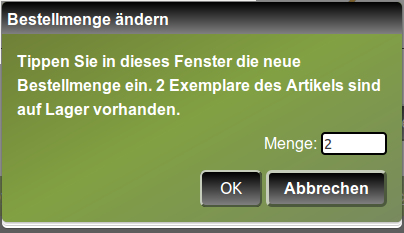
\includegraphics[width=70mm]{Bilder/mengenaenderung.png}
	\end{center}
	\caption{Dialog: Bestellmenge ändern}
\end{figure}

\textbf{Löschen eines Artikels aus dem Warenkorb}\\
Um ein Artikel aus dem Warenkorb zu löschen, wurden zwei Methoden umgesetzt. Bei der ersten Methode handelt es sich um einen Hyperlink, der sich hinter jeder Artikelzeile auf der Warenkorbübersichtsseite befindet. Der Hyperlink wird auf der Seite durch ein rotes Kreuz dargestellt. Dieser Hyperlink lädt die Seite neu und übergibt als Parameter, dass der Artikel mit der Artikelnummer X gelöscht werden soll. Die Datei \glqq /Funktions/warenkorb.php,inc\grqq{} nimmt wieder den Parameter entgegen und ruft ein Dialog-Fenster auf (siehe \textit{Abbildung 39}). Beim Dialog-Fenster muss der Kunde bestätigen, dass wirklich der Artikel gelöscht werden soll. Der \glqq OK-Button\grqq{} des Dialogs ist mit einen Hyperlink gelöst worden. Dieser Hyperlink lädt die Seite neu und übergibt als Parameter, dass der Artikel wirklich gelöscht werden soll. Die Datei \glqq /Funktions/warenkorb.php,inc\grqq{} erkennt den gesetzten Parameter und ruft die Methode \glqq entferne\_artikel\_aus\_warenkorb(\$pid)\grqq{} der Klasse \glqq Warenkorb\grqq{} auf. Diese Methode löscht den Artikel aus dem Warenkorb. Die Variabel \glqq \$pid\grqq{} enthält bei dieser Methode die Artikelnummer des Artikels, der aus dem Warenkorb gelöscht werden soll.\\
Eine weitere Löschfunktion wurde mit Checkenboxen umgesetzt. Durch die Checkboxen kann der Kunde mehrere Artikel löschen. Der Kunde markiert mit den Checkboxen die Artikel, die gelöscht werden sollen. Durch einen Klick auf den Button \glqq Markierte Artikel löschen\grqq{} wird die Markierung an den Server weitergeleitet. Die Weiterleitung findet über die Methode \glqq POST\grqq{} statt. Bei den Button \glqq Markierte Artikel löschen\grqq{} handelt es sich um einen Submit-Button. Die Checkboxen befinden sich in einen HTML-Formular. Dieses Formular überträgt bei einer Bestätigung des Submit-Buttons die Namen  der markierten Checkboxen und die zugeordneten Artikelnummern an das PHP-Skript \glqq /Funktions/warenkorb.php,inc\grqq{}. Das Skript zeigt nach dem Erhalt der Daten auch ein Dialog mit einer Sicherheitsfrage an. Wird diese Frage bestätigt, sorgt der Bestätigungs-Hyperlink dafür, dass die Methode \glqq mehrere\_artikel\_aus\_warenkorb\_entfernen(\$arr\_pids)\grqq{} der Klasse \glqq Warenkorb\grqq{} aufgerufen wird. Diese Methode löscht alle als Array übergebenen Artikel aus den Warenkorb. Der Parameter \glqq \$arr\_pids\grqq{} enthält somit ein Array mit Artikelnummern der Artikel, die aus dem Warenkorb entfernt werden sollen. Das Array wird aus dem vom Formular übertragenen Daten erstellt.

\begin{figure}[H]
	\begin{center}
			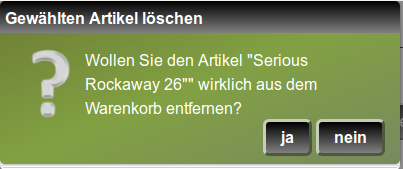
\includegraphics[width=70mm]{Bilder/sicherheitsfrage_artikel_loeschen.png}
	\end{center}
	\caption{Dialog: Sicherheitsfrage Artikel löschen}
\end{figure}

\subsubsection{Zum Teil übernommenes Arbeitspaket: Bestellvorgang}
Da auch der Bestellvorgang etwas hinter dem Zeitplan lag, wurde hier auch ein Teil von Herrn Brüntrup übernommen. Es wurde eine Routine programmiert, die nach dem Klicken des Buttons \glqq Zur Kasse\grqq{} abgelaufen wird. In dieser Routine stellt der Kunde alle Einstellungen, die mit der Bestellung zu tun haben, ein. Hierzu gehört die Versandart, eine nochmalige Möglichkeit den Warenkorb zu ändern, die Zahlungsart und die Lieferadresse. Die letzte Seite der Bestellroutine zeigt nochmal alle Einstellungen übersichtlich auf einer Seite zusammen gefasst. Auf dieser Seite können alle Einstellungen nachträglich verändert werden. Die Übersichtseite entspricht somit den Gesetz des bürgerlichen Gesetzbuches §312g Absatz 1. Bei diesem Gesetz muss dem Kunden die Möglichkeit gegeben werden, nochmal vor dem Absenden der Bestellung alle Einstellungen bezüglich der Bestellung ändern zu können. Bei online Shops existiert auch eine \glqq Ausgestaltungspflicht des Bestellbuttons\grqq{}. Der Button zum Bestellabschluss muss aus den anderen Button hervorstechen und eindeutig beschriftet sein. Es muss also den Kunden klar werden, dass die Bestellung mit den Button abgeschlossen wird und diese kostenpflichtig ist. Bei diesem Webshop wurde der Button deswegen in einer anderen Farbe gefärbt und mit \glqq Jetzt kostenpflichtig bestellen\grqq{} beschriftet. Der Kunde kann allerdings nur die Bestellung abschließen, wenn dieser die AGB des Webshop akzeptiert hat. Somit wird die AGB ebenso auf der Bestellübersicht angezeigt. Akzeptieren kann der Kunde die AGB indem dieser bei der Checkbox \glqq Ich akzeptiere die AGB.\grqq{} einen Hacken setzt. Wie auf der \textit{Abbildung 37} zu sehen ist, wurde bei der Übersichtsseite die Änderungsfunktionen über einen Hyperlink mit Stiftsymbol umgesetzt. Dieser Hyperlink leitet den Kunden zu der Seite der Bestellroutine zurück, wo die entsprechende Einstellung getätigt wurde.

\begin{figure}[H]
	\begin{center}
			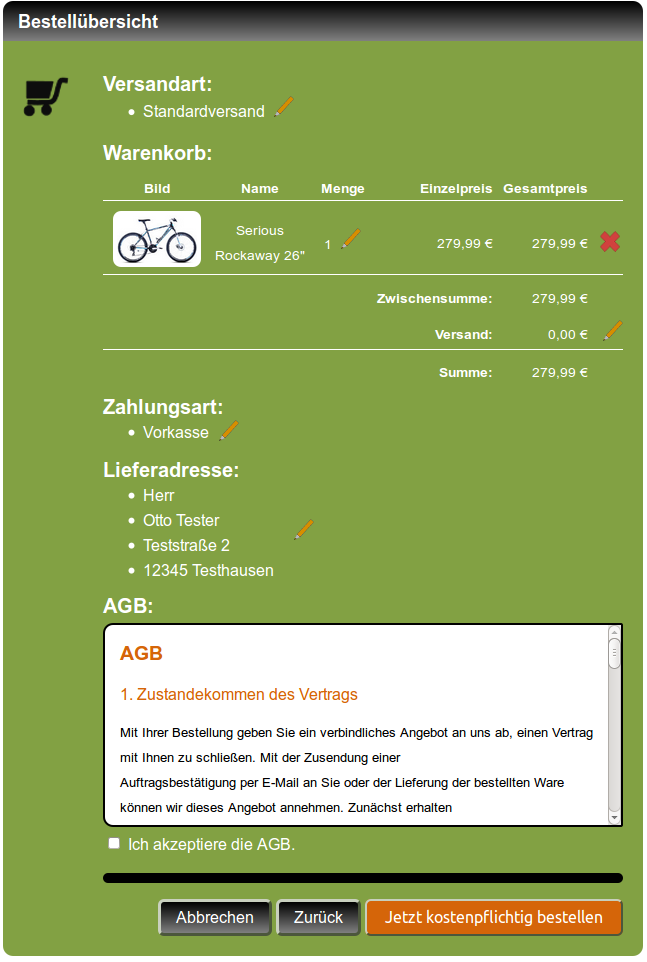
\includegraphics[width=100mm]{Bilder/bestelluebersicht.png}
	\end{center}
	\caption{Bestellroutine: Bestellübersicht}
\end{figure}

Beim Klicken auf dem  Bestellbutton wird die Seite neugeladen. Die neugeladene Seite ruft nun die Methode \glqq zwischengespeicherter\_bestellungslisteneintrag\_bestellen()\grqq{} auf, welche der Klasse \glqq Bestellungen\grqq{} angehört. Diese Methode schließt den Bestellvorgang ab und speichert alle Einstellungen auf der Datenbank ab. Da es gesetzlich vorgeschrieben ist, dass unverzüglich nach dem Absenden der Bestellung diese bestätigt werden muss, versendet der Webshop somit sofort eine Bestätigungs-Email. Zum Absenden der Bestätigungs-Email wurde ebenfalls eine Methode in der Klasse \glqq Bestellungen\grqq{} angelegt. Der Name dieser Methode lautet \glqq sende\_bestaetigungs\_email()\grqq{}. Als Content-Type der Email wurde HTML festgelegt. HTML bietet den Vorteil, dass die Email in den Design des Webshops gestaltet werden konnte und auch Tabellen, Farben und Bilder anzeigen kann. Über die eigentlichen HTML-Ansicht der Email wurde die Style-Anweisung der Email gepackt. Somit muss diese nicht erst vom Webserver geladen werden, wenn der Kunde die Email aufruft. Für das Versenden der Email ist eine andere Klasse zuständig. Der Name dieser Klasse lautet \glqq Email\grqq{}. In dieser Klasse wurde eine Methode implementiert, die sofort schon den richtigen Header für eine Email mit den Content-Type \glqq HTML\grqq{} schreibt und diese über die, in der \glqq Config-Datei\grqq{} festgelegte Email-Adresse versendet. Der Name dieser Methode lautet \glqq html\_email\_senden(\$empfaenger\_adresse, \$betreff, \$html\_code)\grqq{}. Die \textit{Abbildung 38} zeigt einen Ausschnitt der Bestätigungs-Email.

\begin{figure}[H]
	\begin{center}
			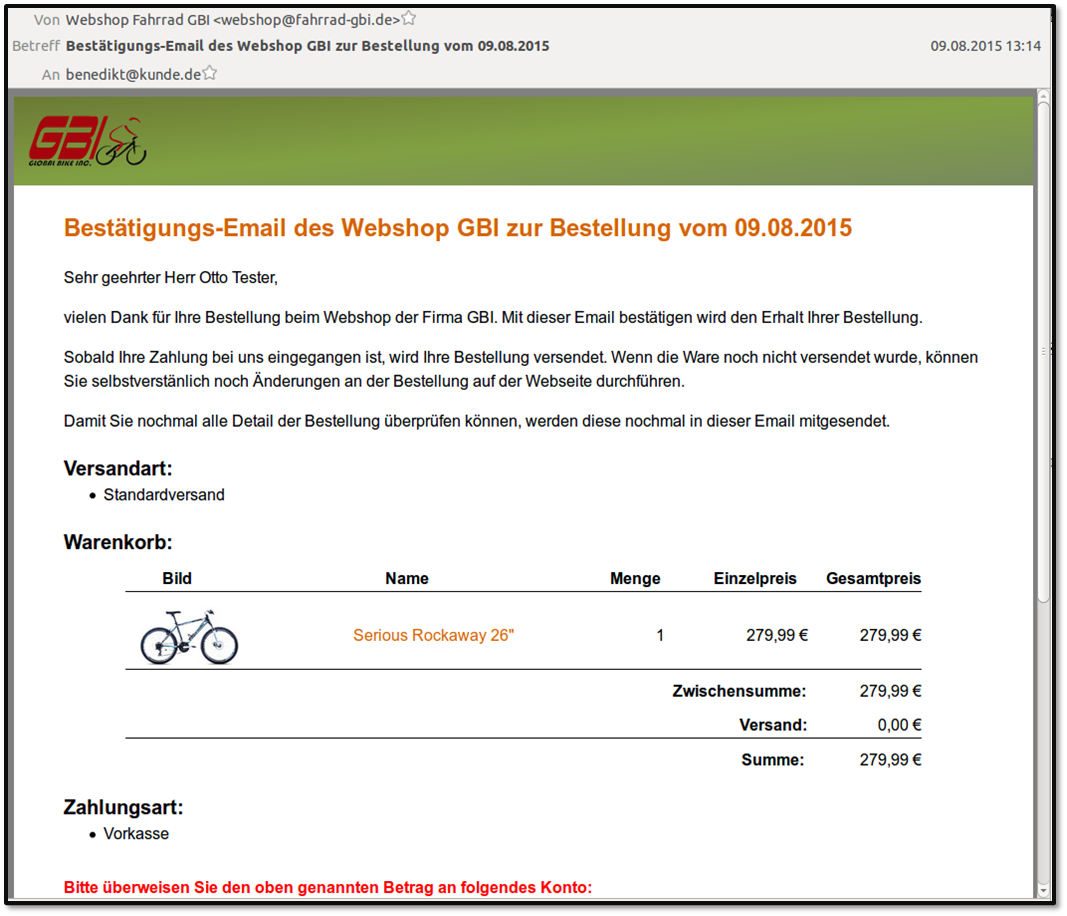
\includegraphics[width=125mm]{Bilder/email.png}
	\end{center}
	\caption{Bestätigungs-Email}
\end{figure}

\textbf{Seiten der Bestellroutine}\\
Mit der Übersichtseite inbegriffen besteht die Bestellroutine aus fünf Seiten. Damit die Webseite möglich übersichtlich gestaltet ist, wird deswegen auf jeder Seite nur eine Einstellung vorgenommen. Bei der ersten Seite wird z.B. nur die Versandart festgelegt. Sind für die Einstellung Eingabefenster nötig, so werden diese, wie schon mehrfach erklärt client- und serverseitig überprüft. Es wurde sich dazu entschlossen immer nur eine Einstellung auf eine Seite zu packen, da bei bestehenden Anbietern, wie z.B. Amazon das \glqq Vollpacken\grqq{} der Seiten der Bestellroutine als sehr unübersichtlich angesehen wurde. 

\newpage
\subsection{Arbeitspakete von Raphael Gregarek$^3$}
Im folgenden Abschnitt wird behandelt, wie Herr Gregarek den Marketing Mix, den Warenkorb, sowie den Bestellvorgangsprozess gelöst hat.

\subsubsection{Arbeitspaket 8: Warenkorb}
Zu Beginn wurde sich über die Funktionen und das Design des Warenkorbs Gedanken gemacht. Ziel war es, das die nötigen Funktionen verfügbar sind, zum Beispiel das Anzeigen von Artikeln mit diversen Eigenschaften sowie die Möglichkeit die Menge zu ändern als auch den Artikel vollständig aus dem Warenkorb zu entfernen. Dies wurde auch mit den anderen Gruppenmitgliedern kommuniziert, sodass mit der Programmierung des Warenkorbs fortgefahren werden konnte. Die \textit{Abbildung 34} zeigt das fertige Design des Warenkorbs. Es befinden sich noch 2 Buttons am unteren Ende die ermöglichen Artikel zu löschen oder den Bestellvorgang zu starten.\\

\textbf{Flyout Warenkorb}\\
\begin{figure}[H]
	\begin{center}
			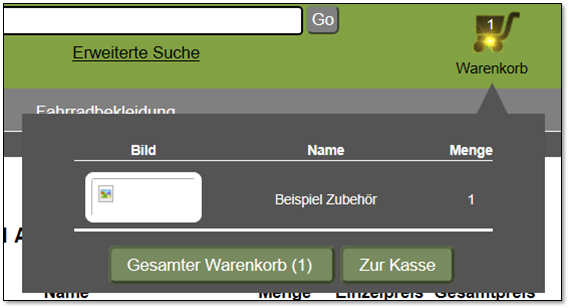
\includegraphics[width=95mm]{Bilder/warenkorb_flyout.png}
	\end{center}
	\caption{Flyout Warenkorb}
\end{figure}

Ähnlich wie die Profilverwaltung sollte auch der Warenkorb als Flyout aufrufbar sein um eine schnelle Ansicht der sich darin zu befindenden Artikel zu zeigen (siehe \textit{Abbildung 39}). Auch hier befinden sich wieder 2 Buttons. Der erste Button ermöglicht es den gesamten Warenkorb anzuzeigen. Dies ist aus dem Grund interessant, weil das Flyout unter Umständen nicht alle Artikel anzeigt. Das liegt daran, da das Flyout nur zur Übersicht sollte es klein sein und bei einer längeren Bestellung müsste man unter Umständen runterscrollen um den gesamten Warenkorb anzuzeigen. Dies wäre unübersichtlich und wenig hilfreich. Der zweite Button führt weiter zur Kasse, wo die Bestellung abgeschlossen wird. Das Warenkorbsymbol  (siehe \textit{Abbildung 40}) am oberen Teil des Webshops zeigt an, wie viele Artikel sich schon im Warenkorb befinden. Der restliche Teil des Warenkorbs wurde vom Gruppenmitglied Benedikt Brüntrup übernommen.

\begin{figure}[H]
	\begin{center}
			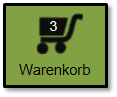
\includegraphics[width=25mm]{Bilder/Warenkorb_symbol.png}
	\end{center}
	\caption{Flyout Warenkorb}
\end{figure}

\subsubsection{Arbeitspaket 9: Bestellvorgang}
Große Teile wurden auch hier von Benedikt übernommen, sodass letztlich noch die Auflistung der bisherigen Bestellungen und die Möglichkeit der Stornierung implementiert wurden. Dazu wurden in der Klasse Bestellungen Methoden mit Datenbankanfragen erstellt. Da das Design im gesamten Webshop gleich ist, konnten die Style Anweisungen zum Teil vom Warenkorb übernommen werden.

\subsubsection{Arbeitspaket 10: Erstellung eines Marketing Mix}
Dieser Teil beschreibt wie der Marketing Mix erstellt wurde, beziehungsweise welche Teilschritte nötig waren um den Marketing Mix umzusetzen.\\
Zu Beginn wurde die Zielgruppe definiert sowie eine Marktanalyse angefertigt. Diese kann als Grundlage für den Marketing Mix angesehen werden und nur so ist es möglich die richtige Strategie für das eigene Unternehmen zu finden. Denn wenn man nicht weiß an wen das Produkt gerichtet ist und vor allem wie die Marktsituation auch in Hinblick auf die Zukunft ist, ist ein Marketing Mix ohne dieses Wissen wahrscheinlich hinfällig beziehungsweise weniger hilfreich. Nur mit einer Vorarbeit lässt sich eine feste Strategie planen, die auch zielführend ist.\\
Danach wurde der Marketing Mix erstellt. Wie für ihn üblich wurden die 4Ps (Produktpolitik, Preispolitik, Distributionspolitik und Kommunikationspolitik) der Reihe nach abgearbeitet. Dabei wurde in der Kommunikationspolitik nur auf die Online Vermarktung eingegangen, da dies auch in der Aufgabenstellung gefordert war. Einzig die Aufgabe nur den Großraum OWL anzusprechen wurde in den Hintergrund gerückt, da es online schwer ist klare Grenzen zu ziehen. Dies wurde auch im Marketing Mix berücksichtigt. \\

\textbf{Marktanalyse – Grundlage des Marketing Mix}\\

\small{\textbf{Die Zielgruppe festlegen}}\\
Als Zielgruppe selber wird jeder Mitbürger definiert, der in der Lage ist ein Fahrrad zu fahren oder eben jenes zu erwerben. Als Gruppe könnte auch nur der Großraum OWL wie in der Aufgabenstellung gefordert wird, als Zielgruppe definiert werden, jedoch ist es aufgrund eines Onlinemarketings und der Betreibung eines Webshops unmöglich nur den Großraum OWL als Zielgruppe zu nennen. Diese beiden Faktoren stehen gerade für die Globalisierung und vergrößern so die Zielgruppe ungemein. Die Grenzen des Webshops sind seine Lieferbedingungen, also die Lieferung der Artikel in bestimmte Länder. Und die GBI beschränkt sich hierbei auf Deutschland. Als weiteren Faktor ist auch die Sprache zu nennen. Denn durch die Wahl der Sprache im Webshop werden schon Menschen ohne deutsche Sprachkenntnisse ausgeschlossen, sodass diese auch nicht die Zielgruppe sein können.
Zu beachten ist auch die Produktplatte, die die GBI zu bieten hat. Sie hat vor allem Sportfahrräder und Mountain Bikes im Angebot. Die Zielgruppe auch wenn dies etwas stereotypisch ist, sind somit jüngere Männer. Natürlich verkauft die GBI die Fahrräder auch an andere Gruppen, jedoch wird der Großteil eben an die eben genannte Gruppe gehen, wobei der Begriff jung sehr weit gefasst werden kann. Gerade im Hinblick auf die E-Bikes kann sich die Käufergruppe sehr schnell ändern.\\

\small{\textbf{Marktgröße}}\\
Hier sind verschiedene Aspekte zu beachten:
\begin{enumerate}

	\item \textbf{Die Marktgröße – wie groß ist der Markt in der Gegenwart}
	\begin{figure}[H]
		\begin{center}
			\fbox{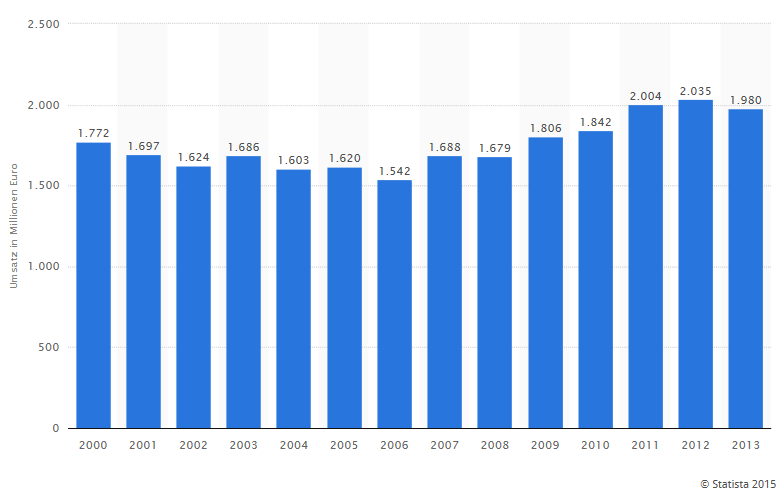
\includegraphics[width=125mm]{Bilder/umsatz_fahrrad_verkaeufe_de.png}}
		\end{center}
		\caption{Umsatz von Fahrradverkäufen in Deutschland}
	\end{figure}
	%Bildquelle: http://de.statista.com/statistik/daten/studie/154152/umfrage/umsatz-durch-fahrradverkaeufe-in-deutschland-seit-2000/
	
Das vergangene Jahr war für den Fahrradmarkt in Deutschland ein sehr starkes und bestätigt den groben Trend im Diagramm. Während von 2000 bis 2006 ein negativer Trend zu beobachten war, ist aber 2007 ein durchweg positiver Weg zu beobachten. Lediglich 2013 war sehr Umsatzschwach. 2014 wurden etwa 4,1 Millionen Fahrräder verkauft (inklusive E-Bikes) was einem Umsatz von 2,16 Milliarden Euro entspricht. Wichtig für die GBI ist auch der E-Bike Markt. In Deutschland gibt es momentan etwa 2,1 Millionen E-Fahrräder.

	\item{\textbf{Marktwachstum und –Dynamik – der Trend des Marktes}}
	
Der Markt ist in einer Wachstumsphase und das besonders bei den E-Fahrrädern. Ein Umsatzplus 2014 im zweistelligen Bereich macht dies deutlich. Aber auch der der Markt für nicht elektrische Fahrräder erfährt ein konstantes Wachstum. Somit erlebt der gesamte Markt einen positiven Trend, der auch von dem oben gezeigten Diagramm bestätigt wird.
Einen gesonderten Blick auf den E-Bike Markt sollte auf jeden Fall geworfen werden. Hier ist ein großes Wachstum in den nächsten Jahren zu erwarten, wenn man die momentane Situation zu Grunde legt. Gegenüber dem Vorjahr ein Plus von 17 Prozent ist eine sehr beachtliche Steigerung. Der Anteil der E-Fahrräder am gesamten Markt beträgt mittlerweile 12 Prozent.

	\item{\textbf{Marktpotenzial – Chancen des Marktes}}
	
Der Fahrradmarkt in Deutschland hat gute Chancen weiter zu wachsen. Dies hat verschiedene Gründe, die in sehr unterschiedlichen Bereichen liegen. Zum einen ist die Natur zu nennen. Damit ist gemeint, dass viele Menschen ihre Lebensweise ändern um die Natur weniger zu belasten. Das fängt damit an den Weg zur Arbeit mit dem Rad zu fahren. Dies tun einige der Natur zur Liebe andere sparen sich somit das Benzin, das für das Auto nötig wäre oder das Ticket für die Bahn oder den Bus. Das Fahrrad wird auch gerne als Sportmittel genutzt oder einfach dafür sich in der Umwelt zu bewegen.
Chancen sind vor allem im E-Fahrrad Markt. Mittlerweile werden auch jüngere Menschen mit anderen Modellen wie E-Mountainbikes angesprochen, was großen Anklang findet.
Die Entwicklung von E-Bikes sollte auch kritisch betrachtet werden. Im Moment wächst der Markt stetig, da es ein relatives neues Produkt ist. Die Gefahr, dass es nur eine Blase ist, die in naher Zukunft platzt ist eine durchaus denkbare  Möglichkeit. Jedoch sieht der momentane Blick in die Zukunft rosig aus, was das sehr starke Wachstum des E-Bike Marktes bestätigt. Dennoch muss immer im Blick sein, dass das Interesse nach E-Bikes sinken könnte.
\end{enumerate}
\textbf{Marketing Mix}\\

\small{\textbf{Aufgabenstellung}}\\
Dieser Abschnitt behandelt den Marketing Mix für den Großraum OWL. Bei dem Marketing Mix wurde besonders aufgrund des Webshops auf die Online-Vermarktung eingegangen.\\

\small{\textbf{Produktpolitik}}\\
Die GBI hat schon eine breite Palette an Fahrrädern und Zubehör zu bieten. Lediglich der Bereich der E-Bikes wird momentan erschlossen. Das Design sollte ähnlich den der bisherigen Modelle gewählt werden um auch bei den neuen Produkten einen Wiedererkennungswert zu generieren. Wenn möglich sollte das Fahrrad bzw. E-Bike das gleiche Aussehen haben und sich nur durch die notwendigen Eigenschaften unterscheiden, was ein E-Bike zu einem E-Bike macht.\\
Da der Webshop neu ist, könnte das Verpackungsdesign an das Unternehmen angepasst werden. Den Namen der Firma oder das Logo selber könnte an der Außenseite zu finden sein. So kann man sich von der Konkurrenz absetzen und schon beim bloßen Ansehen des Pakets wird das Unternehmen GBI sichtbar. Jedoch ist auch auf eine schlichte Verpackung zu achten, da die GBI Qualität vorlebt und dies muss nicht durch ein übertriebenes Verpackungsdesign zu Nichte gemacht werden.\\

\small{\textbf{Preispolitik im Marketingmix}}\\
Für die Preispolitik muss die GBI einige Faktoren berücksichtigen bevor sie sich letztendlich festlegt. Die GBI ist im Fahrradbereich ein bekanntes Unternehmen und in Teilbereichen sogar weltweiter Marktführer. Die Bereiche sind Sporträder und Mountain Bikes im Privatkundenumfeld und im geschäftlich öffentlichen Umfeld, der Spitzensport. Damit ist die GBI nicht gezwungen eine aggressive Preisstrategie zu fahren um Bekanntheit zu erlangen. Dies ist auch ein enormer Vorteil der GBI. Sie kennen den Markt schon und wissen durch ihre Erfahrung welcher Preis der Kunde bereit ist für ihre Produkte zu zahlen.

Der Webshop ist allerdings ein neuer Teilbereich und so sollten wenigstens für einen bestimmten Zeitraum besondere Angebote für Fahrräder und Ersatzteile gemacht werden. Der Webshop besitzt auf der Startseite schon erste Angebote. Dies sollte auch auf bestimmte Zeit so fortgeführt werden. Der Slogan \glqq Fahrrad des Tages\grqq{} generiert eine besondere Stellung des Fahrrads im Webshop und lenkt die Aufmerksamkeit auf dieses Produkt.

Der Verbraucher hat durch das Internet die Möglichkeit die Preise für jedes Produkt zu vergleichen und die GBI muss sich in diesem Bereich neu aufstellen, da Sie hier noch nicht mit einem eigenen Webshop vertreten war. Angebote helfen hierbei die Marke im Internet bekannter zu machen. Zu beachten ist jedoch auch die Philosophie für die, die GBI, steht. Der Fokus des Unternehmens ist auf Qualität, Stärke und Leistung festgelegt. Dies bedeutet auch, dass der Kunde von vornherein erwarten kann ein einwandfreies, qualitativ hochwertiges Produkt zu bekommen. Der Preis sollte sich also nicht im unteren Bereich des Marktes befinden. Dafür ist der Name zu bekannt, als das die GBI hier einen Preiskampf fahren muss. Der Webshop hat auch einen nicht unwichtigen Vorteil gegenüber z.B. Fahrradgeschäften. Der Verkaufsraum beziehungsweise auch der Verkäufer oder Ausstellungsstücke fallen im Internet weg. So spart man beachtliche Kosten die eine Drückung des Preises nach unten ermöglichen.

Die Kategorie E-Bikes ist ein neuer Bestandteil der Produktpalette und die GBI muss sich hier noch beweisen, dass sie auch in der Lage sind die gewohnten GBI Standards auf die neuen Produkte zu übertragen. Preislich sollte die GBI hier auch die direkten Konkurrenten im E-Bike Premiumsegment unterbieten um möglichst schnell einen Marktanteil zu generieren.

Die GBI sieht im Webshop zwei Liefermöglichkeiten. Zum einen der Standardversand. Die Kosten betragen üblicherweise 4€. Übersteigt der Wert der gekauften Waren eine bestimmten Wert, im Falle hier 25€, so fallen die Versandkosten weg. Die Idee beruht darauf, den Kunden nach Möglichkeit zu einem größeren Einkauf zu locken, um doch noch den festgelegten Wert zu überschreiten. Dies ist vor allem bei kleineren Produkten wie zum Beispiel bei Zubehör der Fall. Der kostenfreie Versand ist ein Anreiz mehr einzukaufen als man es eigentlich vorhatte. Die zweite Liefermöglichkeit ist für die GBI typisch. Es wird ein Expressversand für 13€ angeboten, der eine sehr schnelle Lieferung garantiert. Im Hinblick auf die Kernkompetenzen des Unternehmens, Qualität und Leistung,  ein guter Schritt, da diese beiden Kompetenzen weiter ausgebaut werden können. Bei den Zahlungsbedingungen geht die GBI kein Risiko ein und vertraut der Vorkasse und dem Bankeinzug. Der Bankeinzug ist vor allem im Deutschen Raum eine sehr beliebte Zahlungsart, weil hier der Kunde lediglich einmalig seine Bankdaten hinterlegen muss, auch wenn er mehrere Bestellungen tätigt und das Unternehmen selbst das Geld von dem Konto des Kunden abbucht.\\

\small{\textbf{Distributionspolitik}}\\
Bei der Distributionspolitik gibt es drei Wege das Angebot an der Kunden zu tragen. Die Möglichkeiten sind über Vermittler, Franchise oder als Direktvertrieb. Durch den neugeschaffenen Standort Höxter und den damit verbundenen Webshop fallen sowohl das Franchise als auch der Vermittler weg. Der Direktvertrieb bietet eine wahnsinnige Kundennähe und eine intensive Beratung. Vor allem bei Fahrrädern ist dies eine gute Idee, da diese sich teilweise sehr unterscheiden, und so kann der Kunde individuell beraten werden. Das fördert den Kundenkontakt und so auch auf Wünsche/Verbesserungen der Kunden eingegangen werden. Ein weiterer nicht unwichtiger Punkt, der für den direkten Vertriebsweg spricht, sind die Kosten. Sowohl Vermittler als auch Franchiseunternehmen möchten Geld verdienen und dadurch muss bei gleichbleibendem Gewinn der Verkaufspreis angehoben werden. Durch das Wegfallen dieser Kosten hat die GBI verschiedene Möglichkeiten das eingesparte Geld zu nutzen. Generell günstigere Preise oder gleichbleibende Preise bei einer höheren Gewinnspanne, vorausgesetzt die abgesetzte Menge bleibt gleich.

\begin{figure}[H]
	\begin{center}
			\fbox{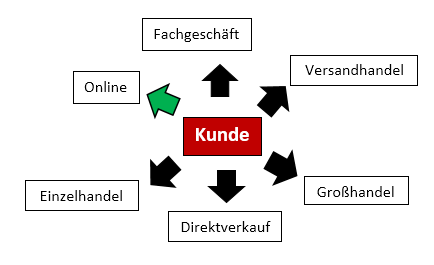
\includegraphics[width=90mm]{Bilder/vertriebskanaele.png}}
	\end{center}
	\caption{Die Vertriebskanäle im Überblick}
\end{figure}

Der nächste Schritt ist die Festlegung des Vertriebskanals der GBI. Hier sollte die Wahl auf dem Onlinehandel liegen. Der eigens angelegte Webshop eignet sich hervorragend um die Produkte der GBI anzubieten. Dafür wurde dieser schließlich angelegt. Die Angebote des Tages auf der Hauptseite sind eine gute Möglichkeit vor allem zur Eröffnung des Shops um möglichst viele Kunden auf die Webseite zu locken, damit der Bekanntheitsgrad steigt. Hier spielt auch der \glqq Click-Counter\grqq{} mir rein, der die Anzahl der Seitenaufrufe zeigt. Somit ist der Webshop möglicherweise bei Suchmaschinen schneller zu finden, da er schon viele Aufrufe generiert hat.

Die GBI muss jedoch auch bedenken, dass die Festlegung auf nur einen Vertriebsweg durchaus problematisch werden könnte. Sie ist durch den einen Vertriebsweg sehr abhängig von ihm. Daher sollte man nach Start des Shops die Verkaufszahlen beachten und den Markt weiter beobachten, ob es nicht sinnvoll wird, den einen oder anderen Vertriebskanal dem Unternehmen hinzuzufügen. Positiv bei der Wahl auf nur einen Kanal zu setzen ist die Tatsache, dass dies enorme Kosten spart. Denn bei den anderen Vertriebswegen gibt es immer mindestens eine handelnde Instanz, die Kosten verursacht, sei es nun das Fachgeschäft oder der Versandhandel.

\begin{figure}[H]
	\begin{center}
			\fbox{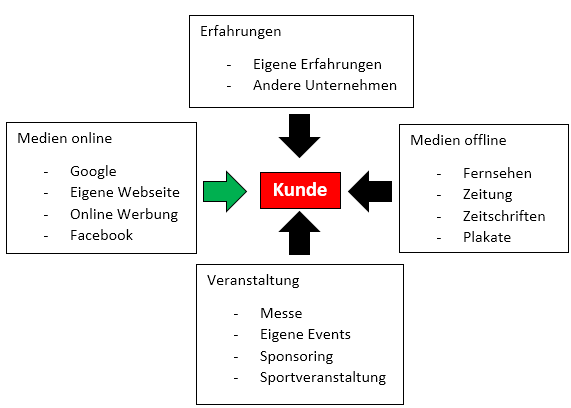
\includegraphics[width=90mm]{Bilder/Werbemoeglichkeiten.png}}
	\end{center}
	\caption{Werbemöglichkeiten im Überblick}
\end{figure}

\small{\textbf{Kommunikationspolitik}}\\
Die GBI wird von vornerein auf die Online Vermarktung setzen. Dies ist eine klare Ausrichtung. Dadurch wird die Kommunikationspolitik lediglich dieses Thema behandeln.

Die Marke GBI ist bekannt. Dies liegt daran, dass die Produkte der GBI in Spitzensport genutzt werden und dadurch die Öffentlichkeit aufmerksam wurde. Zudem sollten wieder die Kernkompetenzen genutzt werden. Qualität und Leistung. Dafür steht die GBI und das müssen auch potentielle Kunden wissen. Daraus resultiert auch die Vorgabe für die Werbung. Die Produkte sind qualitativ hochwertig und nicht minder sollte die Vermarktung sein. Das bedeutet zwar höhere Marketingkosten, jedoch ist das für das Image wichtig, da Kunden sowas miteinander assoziieren. Das Online Marketing kann auf verschiedene Weise genutzt werden. Durch die Festlegung der Zielgruppe im oberen Abschnitt, fällt die Vermarktung leichter. Denn nur wenn die GBI weiß, wer als Kunde geeignet ist, kann sie passgenau für ihre Produkte werben. Die GBI hat nun verschiedene Möglichkeiten ihre Produkte beziehungsweise den Webshop online zu vermarkten. Im Folgenden befindet sich eine grobe Übersicht:
\begin{enumerate}
	\item Marketing über E-Mail
	\item Marketing mithilfe von Suchmaschinen
	\item Schalten von Bannerwerbungen auf Webseiten
	\item Affiliate-Marketing
	\item Social Media Marketing
	\item Einbindung der Produkte in andere Webshops
	\item Der eigene Webshop beziehungsweise die eigene Webseite
\end{enumerate}

Für die GBI scheinen die Kategorien 1, 2, 3 und 5 am sinnvollsten zu sein. Dies ist der Tatsache geschuldet, dass zum einen nicht zwangsweise jede Kategorie beansprucht werden muss und zum anderen das die Kategorien 6 und 7 momentan noch unmöglich beziehungsweise nicht sehr sinnvoll erscheinen. Der Webshop befindet sich momentan im Aufbau und hat noch keine Bekanntheit. Von einer Webseite ist seitens der GBI keine Rede, weswegen diese Möglichkeiten erstmal wegfallen.

Die Marketing Methode über die E-Mail ist im Online Marketing eine lange bekannte und beliebte Variante. Man könnte denken, dass über soziale Netzwerke mehr Menschen erreicht werden aber letztlich ist es so, dass über 95\% der Internetnutzer ein E-Mail Konto besitzen und nur eine weitaus geringere Personenanzahl einen Social Media Account. Darüber hinaus nutzen Menschen nicht nur eine Social Media Seite beziehungsweise sind sie in manchen gar nicht aktiv. Ein E-Mail Konto ist unabhängig vom jeweiligen Anbieter.  Zudem sieht sich ein potentieller Kunde eher eine E-Mail an als einzelne Nachrichten auf einer Social Media Seite, wo förmlich eine Nachrichtenflut herrscht. Das wichtigste für die GBI ist einen Stamm an E-Mail Adressen aufzubauen. Wie dies für die GBI geschieht muss sie selber wissen. Über Offline Events können E-Mail Adressen gesammelt werden aber auch über die eigene Webpräsenz. Oder über die Social Media Seiten der Firma. Wichtig ist, dass vom potentiellen Kunden eine Einwilligung geholt wird. Rechtlich ist die GBI auf der sicheren Seite wenn sie nach dem Double Opt-In Verfahren arbeitet. Zusätzlich sollte noch das Impressum in der Mail vorhanden sein, sowie eine Möglichkeit sich wieder vom Newsletter abzumelden. Über die E-Mail Methode weiß die GBI, dass sie Kunden anspricht, die auch wirklich reges Interesse an dem Produkt zeigen, da sie sich für den Newsletter extra angemeldet haben.

Die zweite Möglichkeit ist die der Suchmaschinen. Bevor die GBI auf den ersten Seiten der Suchergebnisse erscheint wird dies etwas dauern. Beschleunigen lässt sich dies mit den AdWords von Google. Mit AdWords kann sich die GBI Stichwörter kaufen. Wenn nach diesem Stichwort nun gesucht wird taucht die GBI weiter oben in den Suchergebnissen auf. Je nach Stichwort kann dies aber ein teures Unterfangen sein. Zudem dauert es zu Start des Marketings mit AdWords einige Zeit bis die GBI vorne auftauchen wird. Eine andere Möglichkeit ist die der Search Engine Advertising (SEA). Hier bezahlt die GBI für eine Anzeige die neben den Suchergebnissen auftaucht. Gerade zu Beginn eine sinnvolle Alternative, da sich die Anzeige schon auf der ersten Suchergebnisseite befinden könnte. Letztlich sollte die GBI aus einer Mischung aus beidem abzielen. Jedoch kosten beide sehr viel Geld aber bieten ein enormes Potenzial.

Die nächste Art des Online Marketings ist die der Bannerwerbung. Grob unterschieden wird hier zwischen statischen, HTML-, Bild- und Text- sowie animierten Werbebannern. Es gibt sicherlich noch weitere Varianten, doch die eben genannten sind die Bekanntesten. Die Werbung wird auf beliebigen Webseiten geschaltet. Für die GBI bieten sich natürlich Fahrradseiten an, auch die im Bereich des Spitzensports. Im Sinne der Region OWL sollte auch auf regionalen Webseiten mit Bannern geworben werden. Je nachdem wie oft der Banner erscheint oder auf ihn geklickt wird, erhöhen sich die Kosten. Für die Webseiten der Region OWL sollte die GBI aber definitiv über die Bannerwerbung nachdenken.

Für das Social Media Marketing ist generell ein eigener Auftritt beziehungsweise eine eigene Seite sinnvoll. Die großen beiden Vertreter in der Branche sind Facebook und Twitter. Unabhängig auf welcher Seite sich die GBI nun präsentieren wird muss sie aktiv ihre Seite betreiben. Die eigene Seite ist weniger attraktiv, wenn sie nicht regelmäßig aktualisiert wird oder nur selten genutzt wird. So verlieren Kunden schnell das Interesse und werden den Auftritt nicht länger verfolgen. Besonders in Fahrradforen und Foren im Bereich OWL sollte die GBI auch aktiv werden. Dabei sollte sie nicht nur aktiv Werbung für ihre Produkte machen sondern auch potentiellen Kunden helfen. Das richtige Produkt empfehlen, aufzeigen was das Produkt besser macht aber auch ehrlich sein. So bekommt die GBI auch Feedback und kann dieses nutzen um sich selber ständig zu verbessern. Das Internet ist transparent und Fehltritte können fatale Folgen haben. So ist das Social Media Marketing nicht nur als Verkaufs- und Werbemöglichkeit zu sehen, sondern auch als Feedback- und Entwicklungsplattform. Um sehr schnell eine große Gemeinschaft aufzubauen wird der GBI empfohlen auf den Social Media Seiten fachbezogene Beiträge, Gewinnspiele und Rabattangebote anzubieten. Dies fördert das Wachstum der Gemeinschaft und verschafft in kürzester Zeit eine größere Beliebtheit. Gerade als weltweit agierendes Unternehmen, wie die GBI eines ist, wird sie schnell Zuspruch finden. Doch auch Vorsicht ist geboten. Qualität steht immer vor Quantität und das gerade bei der GBI. Lieber sollte sie in regelmäßigen Abständen die Seite aktualisieren als jede Stunden etwas zu verfassen.\\

\small{\textbf{Fazit des Marketing Mix}}\\
Mit diesem Marketing Mix hat die GBI eine Möglichkeit ihre Bekanntheit im deutschen Raum, insbesondere den Großraum OWL zu erweitern. Es wurden sowohl Chancen als auch Risiken gegenübergestellt und konkrete Punkte angesprochen wie die GBI den Webshop einbinden kann. Die 4Ps wurden nacheinander abgearbeitet und anschließend darauf überprüft, ob sie sich ergänzen oder in verschiedene Richtungen führen. Dabei wurde festgestellt, dass die Strategie in eine Richtung geht und somit mit dem nächsten Schritt weiter fortgefahren werden kann.  Die GBI muss nun ein Marketingbudget festlegen, welches mit dem Marketing Mix vereinbar ist.
